\documentclass[10pt]{article}

%%%%%%%%%%%%%%%%%%%%%%%%%%%%%%%%%%%%%%%%%
%%%%%%%%%%%%%% TYPOGRAPHIE %%%%%%%%%%%%%%
%%%%%%%%%%%%%%%%%%%%%%%%%%%%%%%%%%%%%%%%%

%%%%%%%%%%%%%% TEXT
    \usepackage{polyglossia} %| Für deutsche Sprache & Sonderzeichen
    \setmainlanguage{german} %| 
    \usepackage{microtype} % Für schöneren Blocksatz
    \usepackage{parskip} % Für "deutche" Absätze
    \usepackage[official]{eurosym} % Für Eurozeichen
    \usepackage[locale=DE, per-mode=symbol]{siunitx} % Für Einheiten
    \DeclareSIUnit{\eur}{\mbox{\euro}}
    \usepackage{fontspec}
    % https://tex.stackexchange.com/questions/25249/how-do-i-use-a-particular-font-for-a-small-section-of-text-in-my-document/37251#37251
    \newfontfamily\sansemph{Latin Modern Sans} % Für Titel
    \usepackage{csquotes} % Für deutsche Anführungszeichen
    \newcommand{\form}[1]{#1} % Formeln
    \newcommand{\filepath}[1]{\texttt{#1}}
    \newcommand{\cmd}[1]{\texttt{#1}}
    \newcommand{\eng}[1]{\textit{#1}}
    \newcommand{\feng}[1]{{#1}}

%%%%%%%%%%%%%% MATHE
    \usepackage{amsmath} %| Standard ams packages
    \usepackage{amssymb} %|
    \usepackage{amstext} %|
    \newcommand{\sig}{\textrm{sig}}
    % \newcommand{\tanh}{\textrm{tanh}}
    \newcommand{\netin}{\textrm{net}}

%%%%%%%%%%%%%% TEXTLAYOUT
    \usepackage{geometry} % Für Anpassung der Seitenränder
    \geometry{
    	top=2.5cm,
    	left=2.5cm,
    	right=2.5cm,
    	bottom=2cm,
    	footskip=13.6pt
    }
    \usepackage{fancyhdr} % Kopf- und Fußzeilen
    \usepackage{multicol} % Text in mehreren Spalten
    \newcommand{\threesub}[1]{
        \vspace{1.5ex}
        \noindent {\textbf{#1}}
        \vspace{0.5ex}
    }

%%%%%%%%%%%%%%%%%%%%%%%%%%%%%%%%%%%%%%%%%
%%%%%%%%%%%%%% ABBILDUNGEN %%%%%%%%%%%%%%
%%%%%%%%%%%%%%%%%%%%%%%%%%%%%%%%%%%%%%%%%
    \usepackage{float} % Figure "H" Option zur Positionierung
    \usepackage{caption} % Für custom captions
    \captionsetup{textfont={footnotesize}, labelfont={footnotesize, bf}, position=below, format=plain}
    \usepackage{wrapfig} % Für wrapfigure (Text um Bilder herum)
    \usepackage{graphicx} % Für das Einfügen von Bildern

%%%%%%%%%%%%%%% TIKZ
    \usepackage{tikz}
    \usetikzlibrary{matrix, positioning, calc, %
    decorations.pathreplacing, calligraphy % for curly braces
    }
    \usepackage{circuitikz} % Schaltplan,Schaltzeichen usw.
    \tikzset{big elko/.style={elko=#1, capacitors/width=0.3}}
    \usepackage{pgfplots} % Plots
     \pgfplotsset{compat=1.18} % Neuste Version nutzen

%%%%%%%%%%%%%%% PROGRAMMAUSSCHNITTE
    \usepackage[newfloat=true]{minted}
    \usepackage{xparse} % Für NewDocumentCommand und -Environment
    \usepackage{varwidth}
    \definecolor{bg}{rgb}{0.95,0.95,0.95}
    \SetupFloatingEnvironment{listing}{name=Programmausschnitt, listname=Programmausschnitte}
    % https://stackoverflow.com/a/1390520
    %                             #1     #2       #3 #4 #5
    \NewDocumentEnvironment{code}{O{0.7} O{julia}  m  m}{%
        \VerbatimEnvironment%
        \begin{listing}[H]%
            \centering% also for centering
            \begin{varwidth}{#1\textwidth}%
                \begin{minted}[bgcolor=bg, linenos, breaklines]{#2}%
                    } {%
                \end{minted}%
            \end{varwidth}%
            \caption{#3}%
            \label{#4}%
        \end{listing}%
    }
    \newcommand{\coderef}[1]{Programmausschnitt \ref{#1}}

%%%%%%%%%%%%%%%%%%%%%%%%%%%%%%%%%%%%%%%%%
%%%%%%%%%% QUELLEN & VERWEISE %%%%%%%%%%%
%%%%%%%%%%%%%%%%%%%%%%%%%%%%%%%%%%%%%%%%%
    \usepackage[sorting=none, defernumbers=true]{biblatex} % Für Quellenangaben
    \DeclareFieldFormat[online,misc]{title}{\mkbibquote{#1}} % Titel in Anführungszeichen
    \DeclareFieldFormat{type}{} % Quellen-Typ nicht anzeigen
    \addbibresource{sources.bib} % Quellen laden
    
    \usepackage[bookmarks=true]{hyperref}
    \hypersetup{
        pdftitle={Entwicklung eines Frameworks und eigener Hardware für Brain-Computer-Interfaces},
        pdfauthor={Matteo Friedrich \& Alexander Reimer},
        pdfsubject={},% TODO
        pdfkeywords={KI, AI, neuronale Netzwerke, EEG, Elektroenzephalographie, Jugend Forscht, BCI, Brain-Computer-Interface}
    }

\begin{document}

\pagenumbering{gobble}
\thispagestyle{empty}

\vspace*{10mm}
\begin{center}
    {\Huge \textbf{\sansemph Entwicklung eines Frameworks und eigener Hardware für Brain-Computer-Interfaces}} \\[2mm]
    {\Large Sammlung, Verarbeitung und Analyse unserer Gehirnsignale} \\[4mm]
    
\includegraphics[width=0.8\textwidth]{logo.png} \\[10mm]
    {\huge \textbf{Alexander Reimer, Matteo Friedrich und Mattes Brinkmann}} \\[1em]
    {\LARGE \textbf{Gymnasium Eversten Oldenburg}}
\end{center}

\newpage
\pagenumbering{roman}

\tableofcontents

\section*{Kurzfassung}
In diesem Projekt wollen wir ein Framework für ein Brain-Computer-Interface (BCI) verwirklichen. Dafür entwickeln wir unsere eigene, deutlich günstigere Alternative des benötigten Messgerätes (EEG), welches mithilfe von Elektroden Spannungsdifferenzen misst, die von Neuronen im Gehirn erzeugt werden. Gleichzeitig versuchen wir anhand einer schwierigen Aufgabe (Erkennung der Gedanken an verschiedene Richtungen) ein allgemein verwendbares Interface zu entwickeln, welches die Verarbeitung der Gehirndaten, die Erstellung eines neuronalen Netzes für die Analyse und die anschließende Verwendung des BCI übernehmen kann. Dieses Interface soll möglichst weit abstrahiert und vereinfacht sein, aber dennoch tiefgreifende Anpassungen leicht ermöglichen, sodass es hoffentlich Anfänger den Bereich näher bringen, aber auch in Zukunft eine gute Grundlage für erfahrene Entwickler bieten kann.

\newpage

\pagenumbering{arabic}

\section{Einleitung}
Ziel des Projektes ist es, ein Framework für BCIs -- Brain-Computer-Interfaces -- zu entwickeln, welches die Erstellung von BCIs vereinfachen soll, indem der Prozess stark abstrahiert wird.
Dabei ist uns wichtig, dass unser Framework trotzdem durch viele Anpassungsmöglichkeiten auch fortgeschrittene Personen ansprechen kann.

BCIs sind Schnittstellen zwischen Gehirn und Computer und sollen Kommunikation zwischen diesen ermöglichen.
Sie können für die bewusste Steuerung von Dingen wie Prothesen, Drohnen und Robotern verwendet werden, aber auch für diagnostische Zwecke, wie die Voraussage von Migränen oder die Erkennung von Gehirnstörungen.
So wird zum Beispiel gerade daran gearbeitet, BCIs zu verwenden, um die Kommunikation von Menschen mit vollständigem Locked-in-Syndrom (CLIS) mit der Außenwelt zu ermöglichen, obwohl diese keinerlei bewusste Muskelkontrolle mehr haben. \cite{BCIChaudhary}
Außerdem lassen sich BCIs mit instrumentelle oder die klassische Konditionierung sogar zur Veränderung unserer Gehirnmuster und -aktivitäten verwenden. \cite{BCIChaudhary}

% Zum Beispiel haben Forscher aus Stanford ein BCI entwickelt, welches in der Lage ist, behinderten Personen die Möglichkeit zu geben, über ihre Gedanken Nachrichten zu schreiben und so kommunizieren zu können. % TODO: keine Quelle!
% Andere Forscher haben es geschafft, Menschen mit vollständigem Locked-in-Syndrom (CLIS) mithilfe eines BCIs wieder die Kommunikation zu ermöglichen, trotz Fehlen von jeglichen willentlichen Muskelbewegungen.
	
Wir hoffen, bei der Erarbeitung unseres Projektes neben dem Erlangen von Erfahrung in diesem interessanten Bereich auch selbst dazu beizutragen.
BCIs sind ein relativ neues Thema und Forschung in diesem Bereich wird, soweit wir gesehen haben, größtenteils durch Forschungsinstitut, Universitäten, etc. durchgeführt.
Gründe dafür sind vermutlich die hohen Kosten eines EEGs, welches gute Daten liefert, sowie die Komplexität und der Aufwand.
Letzteres liegt auch daran, dass Kenntnisse in verschiedenen Bereichen notwendig sind: Programmieren, Künstliche Intelligenz, Psychologie und Gehirn-Physiologie sowie die Technik und Physik hinter einem EEG.

Wir haben uns mit einigen dieser Bereiche beschäftigt und haben uns als Ziel gesetzt, diesen Prozess der Entwicklung eines BCI leichter und zugänglicher zu machen.

Zum einen wollten wir dazu ein eigenes Software-Framework entwickeln. 
Dieses sollte möglichst viele der oben genannten Aufgaben übernehmen und dem Nutzer ein möglichst abstrahiertes Interface bieten, welches z.B. die Aufbereitung der rohen Daten und die Entwicklung und das Trainieren einer künstlichen Intelligenz übernimmt, ohne dass sich der Nutzer erst detailliert mit diesen Themen auseinander setzen muss.

Gleichzeitig sollen aber Anpassungen und Erweiterungen durch den Nutzer leicht umsetzbar sein, da voraussichtlich nicht in jeder Situation die von uns gewählten Verfahren und Parameter passend sein werden.

Dies ist bereits das zweite Jahr, dass wir an BCIs forschen.
Letztes Jahr hatten wir zwar Erfolg darin, ein BCI zu entwickeln, doch dieses hatte drei hauptsächliche Probleme:

\begin{enumerate}
    \item Es konnte zwar unsere gewählte zu erkennende Aktivität (Schließen der Augen) erkennen, doch diese ist sehr simpel -- die meisten anderen Verwendungszwecke eines BCI sind viel komplexer und wären vermutlich nicht möglich gewesen.
    \item Es war nicht nutzerfreundlich, da es kaum dokumentiert war, nicht ohne Weiteres zur Erkennung beliebiger Aktivitäten verwendet oder anders angepasst werden konnte, und schwer in eigenen Programmen zu verwenden war.
    \item Wir haben das Ganglion EEG von OpenBCI benutzt, welches ca. \SI{500}{\eur} gekostet hat und somit zwar verglichen mit anderen EEGs günstig war, aber für uns noch zu teuer.
\end{enumerate}

Probleme 1 und 2 werden durch das bereits beschriebene Framework abgedeckt; jetzt, da wir etwas mehr Erfahrung haben, achten wir mehr auf die Software-Gestaltung anstelle eines eher Proof-of-Concept artigen Programms.

Das dritte Problem, den Preis des EEG, wollen wir \enquote{lösen} indem wir unser eigenes, günstigeres Selbstbau-EEG entwickeln.
% Mit unserem Framework soll also zum Beispiel eine Person, die Interesse an und Wissen über die biologischen Aspekte eines BCIs hat, l

\newpage % damit Stichpunkte nicht über zwei Seiten aufgeteilt sind

\section{Materialien} 

\begin{itemize}
    % \setlength{\itemsep}{-1cm}
    
    \item Gekauftes EEG aus dem letzten Jahr %
        \vspace*{-2ex}
        \begin{multicols}{2} %
        \begin{itemize} %
            \item 4-Kanal Ganglion Board von OpenBCI $\star$
            \item 4x Spike-Elektroden $\star$
            \item Klettband für die Elektroden $\star$
            \item 2x Ohrclips $\star$
            \item Lithium-Polymer-Akku und Ladegerät $\star$
            \item Plastik-Hülle für das Ganglion Board
        \end{itemize}
        \end{multicols}
        \vspace*{-2ex}
    \item Selbstbau-EEG
        \vspace*{-2ex}
        \begin{multicols}{2}
        \begin{itemize}
            \item Raspberry Pi 3B
            \item Analog/Digital-Wandler MCP3208
            \item Instrumentenverstärker AD620AN
            \item 5x Operationsverstärker LM385
            \item Diverse Widerstände
            \item Keramik-/Tantal-/Elektrolytkondensatoren % TODO: welche wurden verwendet?
            \item Steckbrett
            \item Kabel, Drähte, Krokodilklemmen
            \item Netzteil/Batterie($\pm$ \SI{9}{\volt})
            \item Oszilloskop
        \end{itemize}
        \end{multicols}
        \vspace*{-2ex}
    \item Computer: Aorus 15P (Laptop)
    \vspace*{-2ex}
    \begin{multicols}{3}
    \begin{itemize}
        \item CPU: i7-11800H
        \item GPU: RTX 3060
        \item RAM: 64\,GB
    \end{itemize}
    \end{multicols}
    \vspace*{-2ex}
    \item Julia als Programmiersprache für unser Projekt mit den Packages:
    \vspace*{-2ex}
    \begin{multicols}{4}
    \begin{itemize}
        \item LSL.jl
        \item BaremetalPi.jl
        \item FFTW.jl
        \item CSV.jl
        \item BSON.jl
        \item PyPlot.jl
        \item Flux.jl
        \item CUDA.jl
    \end{itemize}
    \end{multicols}
    \vspace*{-2ex}
    \item OpenBCI GUI
    
    % \begin{itemize}
    %     \item Julia als Programmiersprache für unser ganzes Projekt
    %     \item Flux.jl für das neuronale Netz
    %         %\footnote{\href{https://github.com/FluxML/Flux.jl}{https://github.com/FluxML/Flux.jl}}
    %     \item OpenBCI GUI und LSL.jl als Schnittstelle zum OpenBCI-EEG
    %     % \item BrainFlow.jl als Schnittstelle zum OpenBCI-EEG
    %         %\footnote{\href{https://github.com/brainflow-dev/brainflow}{https://github.com/brainflow-dev/brainflow}}
    %     \item BaremetalPi.jl für das Auslesen des Selbstbau-EEG
    %     \item FFTW.jl für die Fast Fourier Transformation
    %         %\footnote{\href{https://github.com/JuliaMath/FFTW.jl}{https://github.com/JuliaMath/FFTW.jl}}
    %     \item CUDA.jl zum effektiven Nutzen einer NVIDIA GPU
    %         %\footnote{\href{https://github.com/JuliaGPU/CUDA.jl}{https://github.com/JuliaGPU/CUDA.jl}}
    %     \item PyPlot.jl zum Plotten
    %         %\footnote{\href{https://github.com/JuliaPy/PyPlot.jl}{https://github.com/JuliaPy/PyPlot.jl}}
    %     \item BSON.jl zum Speichern und Laden von Netzwerken und Metadaten
    %         %\footnote{\href{https://github.com/JuliaIO/BSON.jl}{https://github.com/JuliaIO/BSON.jl}}
    %     \item CSV.jl zum Speichern und Laden von (EEG-)Daten
    % \end{itemize}
\end{itemize}
 
\section{Vorgehensweise}

Für die Entwicklung unseres Framework und EEG haben wir uns ein Ziel gesetzt: Mit diesen ein BCI entwickeln, welches erkennen soll, ob die Testperson gerade an links, rechts oder nichts denkt.
Grund dafür ist, dass wir durch ein konkretes Anwendungsbeispiel fortlaufend sehen können, wie Änderungen die Qualität und Nutzbarkeit des Programms und des EEG beeinflussen, indem wir die Leistung dieses spezifischen BCIs sowie Komplexität und Aufwand dieses Programms, welches unser Framework verwendet, betrachten.

Die Inspiration kam von Harrison \enquote{Sentdex}: Dieser hat auf GitHub einen frei verwendbaren Datensatz an EEG-Daten hochgeladen, die er mit genau diesem Ziel (Erkennung der Richtung) aufgenommen hat. \cite{Sentdex}

Dieses Anwendungsbeispiel passt sehr gut, da es sehr schwer zu erkennen ist und somit viele Verbesserungen benötigt.
Bei einem sehr einfachen Beispiel hätten wir bereits eine perfekte Genauigkeit von 100\% erreicht und könnten somit nicht die Auswirkungen von weiteren Verbesserungen beobachten.

Außerdem haben wir zu diesem Beispiel durch Sentdex bereits EEG-Daten, wodurch wir bereits mit der Entwicklung der Software beginnen konnten, während wir gerade gleichzeitig das EEG entwickelten.

Da Sentdex selbst daran gearbeitet hat, können wir zusätzlich die Qualität unseres eigenen BCI mit seinem vergleichen und so sehen, wie die Leistung unseres allgemeinen Frameworks im Vergleich zu seinem spezifischen Programm ausfällt. 

% Unser Projekt lässt sich in zwei Bereiche einteilen. 
% Zum einen gibt es den neurobiologischen Teil. 
% Er beschäftigt sich damit, wie man Daten über das Gehirn ermitteln und aufbereiten kann. 
% Hierfür nutzen wie einen Elektroenzephalographhen (EEG), um die Gehirnaktivität zu messen, sowie eine Fourier-Analyse (FFT), um die Frequenzen in den Daten zu ermitteln, da sie für das Verständnis der Daten relevant sind.

% Der zweite Teil unseres Projektes ist die künstliche Intelligenz, die die Ergebnisse der FFT nutzt, um Gehirnmuster zu klassifizieren.

\subsection{Elektroenzephalographie}

Bei der Elektroenzephalographie (EEG) werden Elektroden an der Kopfoberfläche platziert. 
Diese können sehr kleine Spannungen messen, die durch Potentialänderungen in Neuronengruppen im Gehirn entstehen und durch den Schädel dringen. 
Eine Elektrode kann nur die Summe aller lokalen Potentialänderungen messen -- sonst wäre eine Elektrode pro Neuron notwendig. 
Man kann also auch nur ungefähr sagen, wo genau im Gehirn eine Potentialänderung stattgefunden hat. 
Mit mehr Elektroden kann jedoch die örtliche Genauigkeit der Daten erhöht werden.

Bei der Messung der Spannung wird immer eine Differenz zwischen einer Elektrode und einem Referenzpunkt gebildet.
Der Referenzpunkt wird zuvor invertiert.

% Dieser ist bei uns das Ohrläppchen, an dem wir eine Elektrode mit einem Earclip befestigt. 
Dabei gibt es zwei Verfahren: Bei der unipolaren Ableitung von Gehirnpotentialen wird ein neutraler Punkt wie ein Ohrläppchen, der von Gehirnströmen unbeeinflusst ist, gewählt. 
Bei jeder Elektrode wird dann die abgeleitete Spannung von dieser abgezogen.
Bei diesem Verfahren haben also alle Elektroden den gleichen Bezugspunkt

Bei der bipolaren Ableitung hat jede Elektrode als Referenz den jeweiligen Nachbarn.
Bei zwei Elektroden gibt es also nur eine Ausgabe, die Differenz der zwei.
Bei drei Elektroden gibt es zwei Ausgaben, einmal die Differenz von Elektroden 1 und 2 und einmal die Differenz von Elektroden 2 und 3. \cite{EEGHausarbeit}

Meistens wird die unipolare Ableitung gewählt, da bei der bipolaren Daten permanent verloren gehen: Zum einen ein Daten-Kanal und zum anderen kann es bei zwei entgegengesetzten EEG-Spannungen (z.B. Elektrode 1 = \SI{7}{\micro\volt}, Elektrode 2 = \SI{-7}{\micro\volt}) zur Auslöschung des Signals kommen. \cite{EEGHausarbeit}

In allen von uns verwendeten EEG-Daten (sowohl extern als auch selbst erzeugt) handelt es sich um unipolar abgeleitete Potentiale.


% Da an dieser Referenzelektrode keine Gehirnaktivität gemessen wird, ist die abgezogen Spannung praktisch 0. % TODO: Wieso dann überhaupt?
% Somit handelt es sich bei um eine unipolare Ableitung, im Gegensatz zu einer bipolaren Ableitung, bei der jeweils die Differenz von zwei Elektroden an der Kopfhaut gebildet wird. % TO/DO: Quelle +  wieso unipolare und nicht bipolare? Antwort von Mattes ;) : Hier erstmal der Link zur Literatur(auf Seite 29 ff. ist die Antwort) https://www.physik.uni-wuerzburg.de/fileadmin/11010700/_imported/fileadmin/11010700/Didaktik/Zulassungsarbeiten/Schriftliche_Hausarbeit_Feser.pdf------> Kurzfassung: Unipolar bedeutet, dass es nur eine Referenzelektrode gibt. Beim bipolaren EEG ist das Spannungspotential immer relativ zur Nachbarelektrode, was bedeutet, dass immer nur die Potentialdifferenzen (Spannung) zwischen zwei Nachbarelektroden gemessen wird, aber nicht zwischen jeweils einer Elektrode und der Referenzelektrode am Ohr. Je nach Verfahren gibt es halt Vor- und Nachteile zwischen diesen beiden Betriebsarten. Die Ableitung des unipolaren EEG-Signals ist einfacher.

Wir untersuchen ereigniskorrelierte Potentiale (EKPs). 
Diese sind bestimmte Spannungsschwankungen (\enquote{Potentiale}), welche in Zusammenhang mit einem internen oder externen Ereignis stehen, wie z.B. einem lauten Ton, einer Körperbewegung oder hoher Konzentration.  % TODO: Überprüfen: Richtungen denken = EKP? 


% \begin{figure}
%     \centering
%     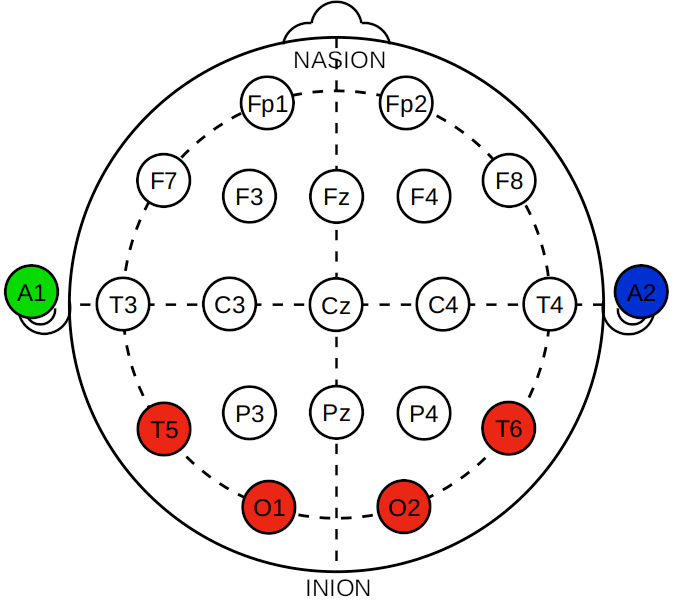
\includegraphics[width=0.5\linewidth]{pictures/Elektroden_Platzierung.jpeg}
%     \caption{10-20 System mit den von uns genutzten Elektroden rot,  Erdungs-Ohrclip grün und \& Referenz-Ohrclip blau gefärbt.}
%     \label{fig:ElektrodenPlatzierung}
% \end{figure}

% \begin{figure}[h!]
%     \centering
%     % TODO: Bild mit richtiger Elektrodenplatzierung (Vis. Cortex), Abb. fig:ElektrodenPlatzierung
%     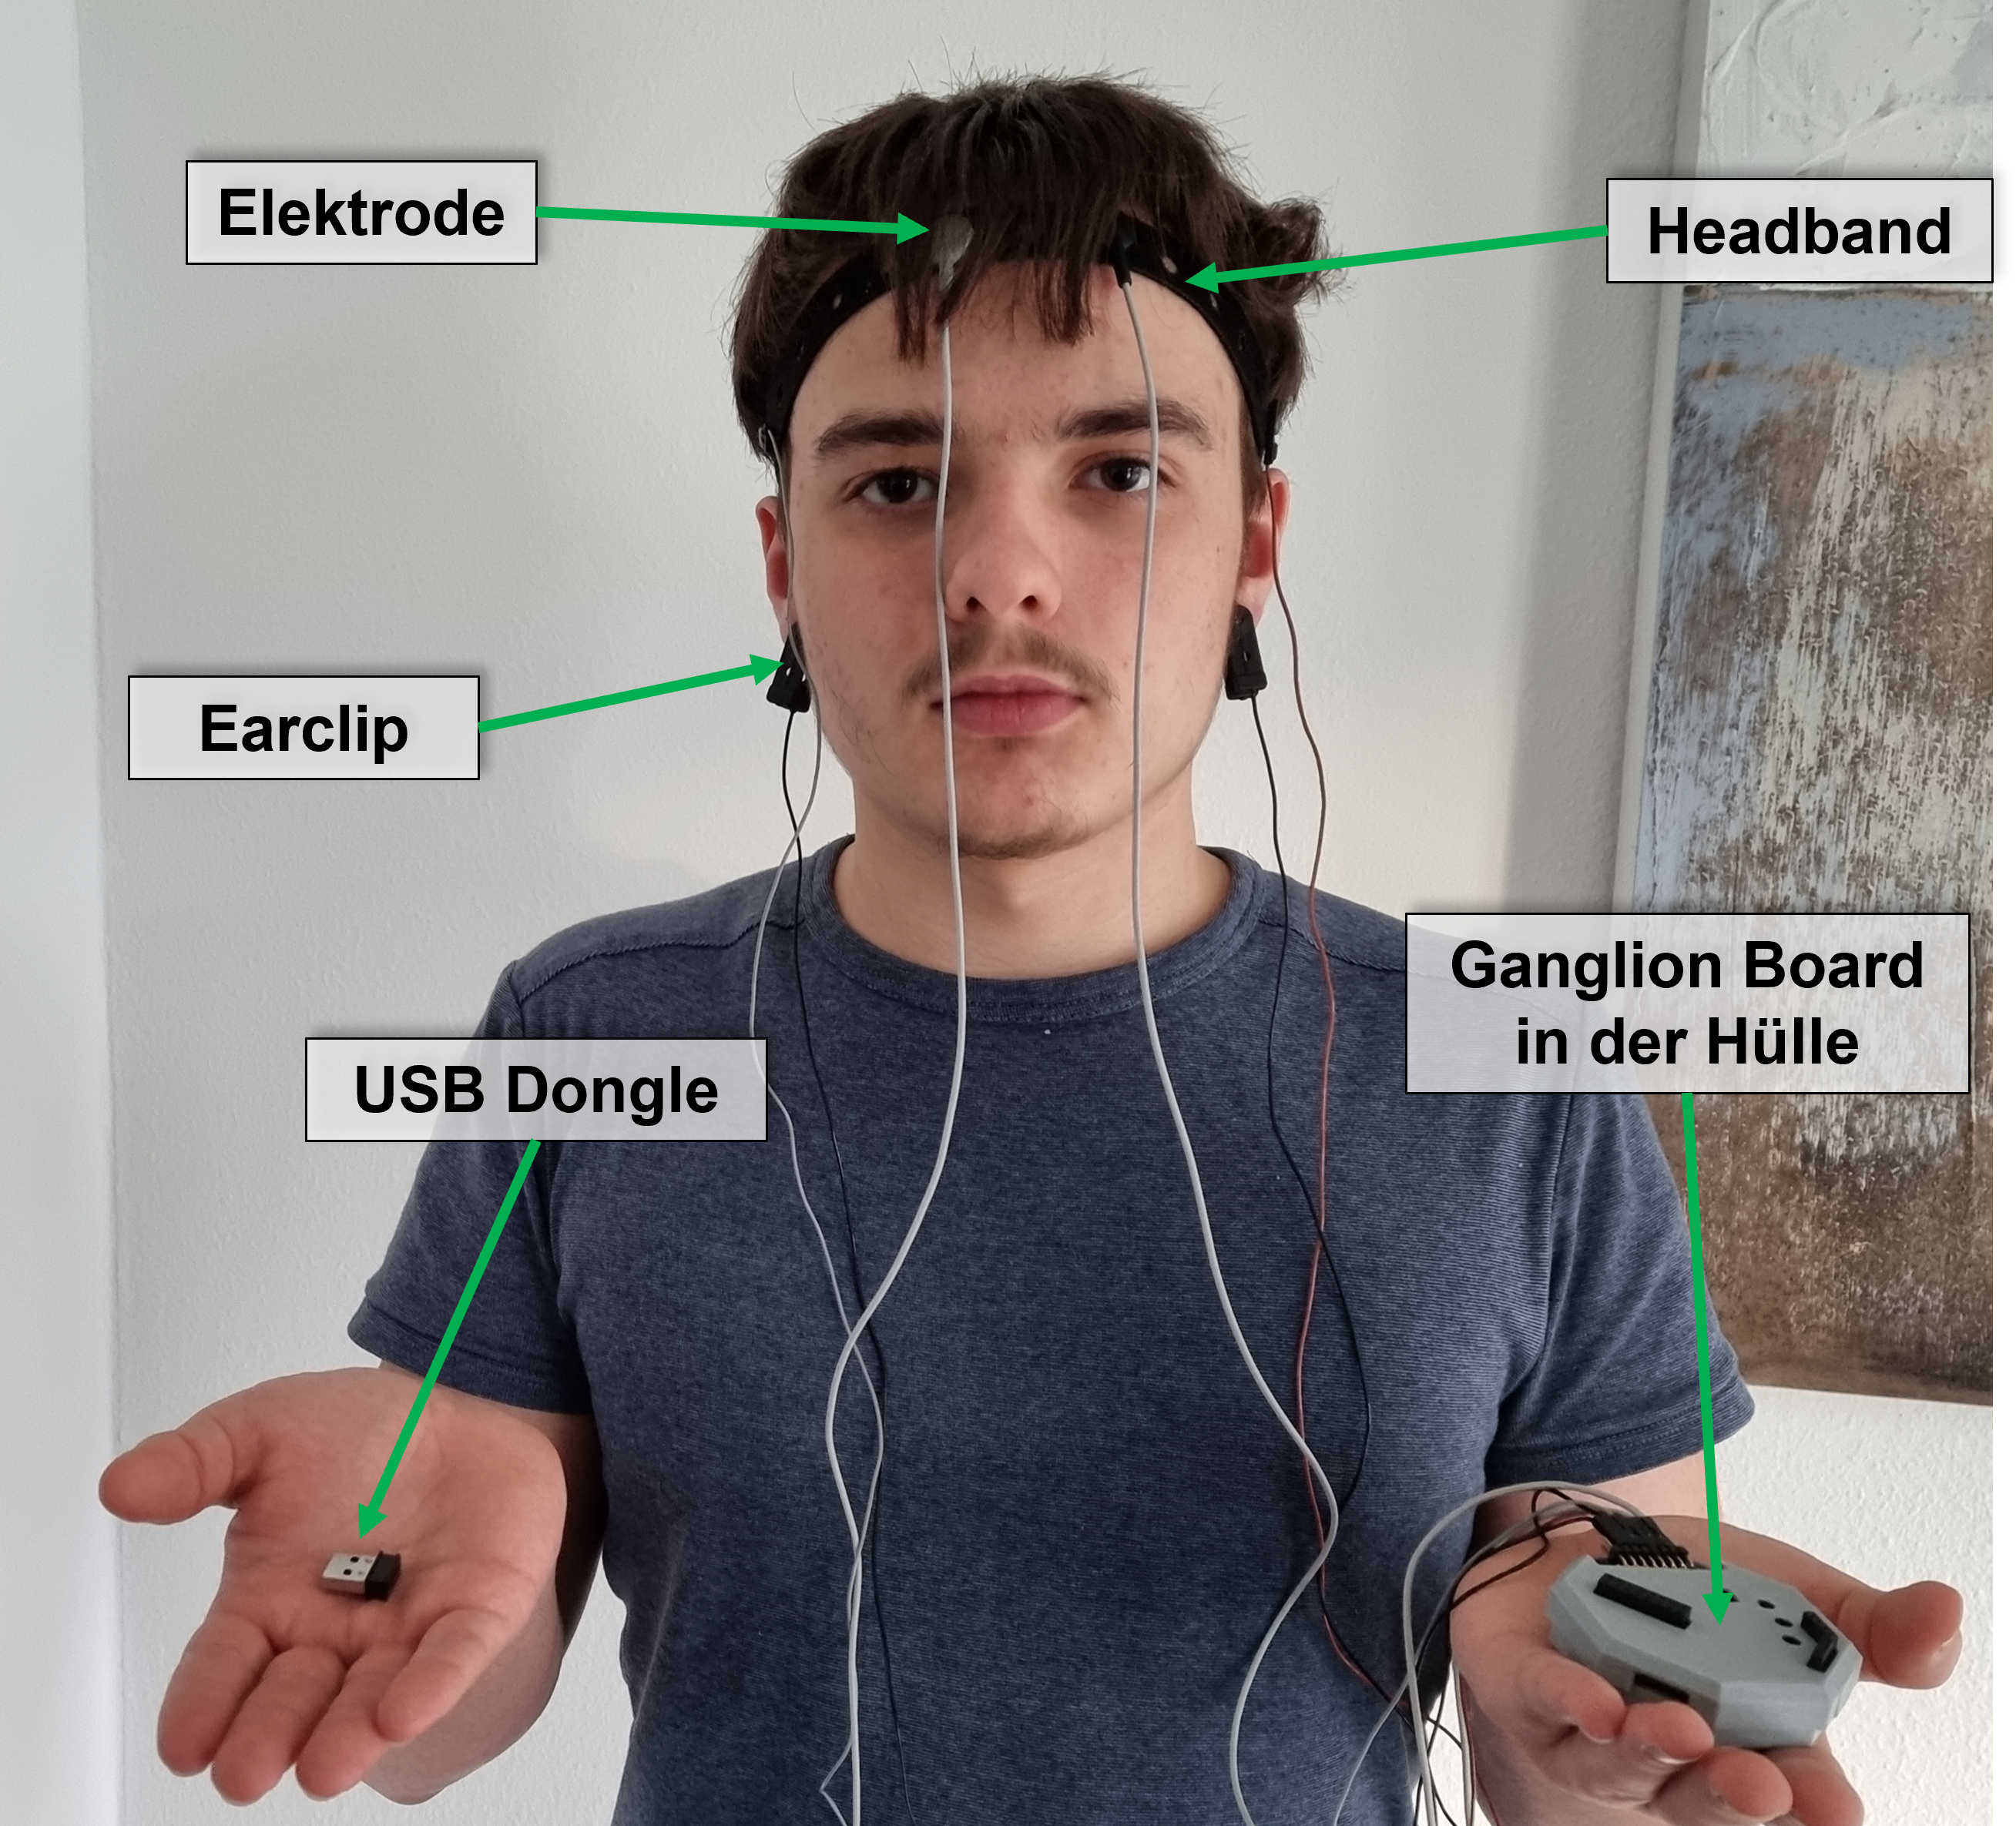
\includegraphics[width=0.46\textwidth]{pictures/EEG-Alex-annotated.png}
%     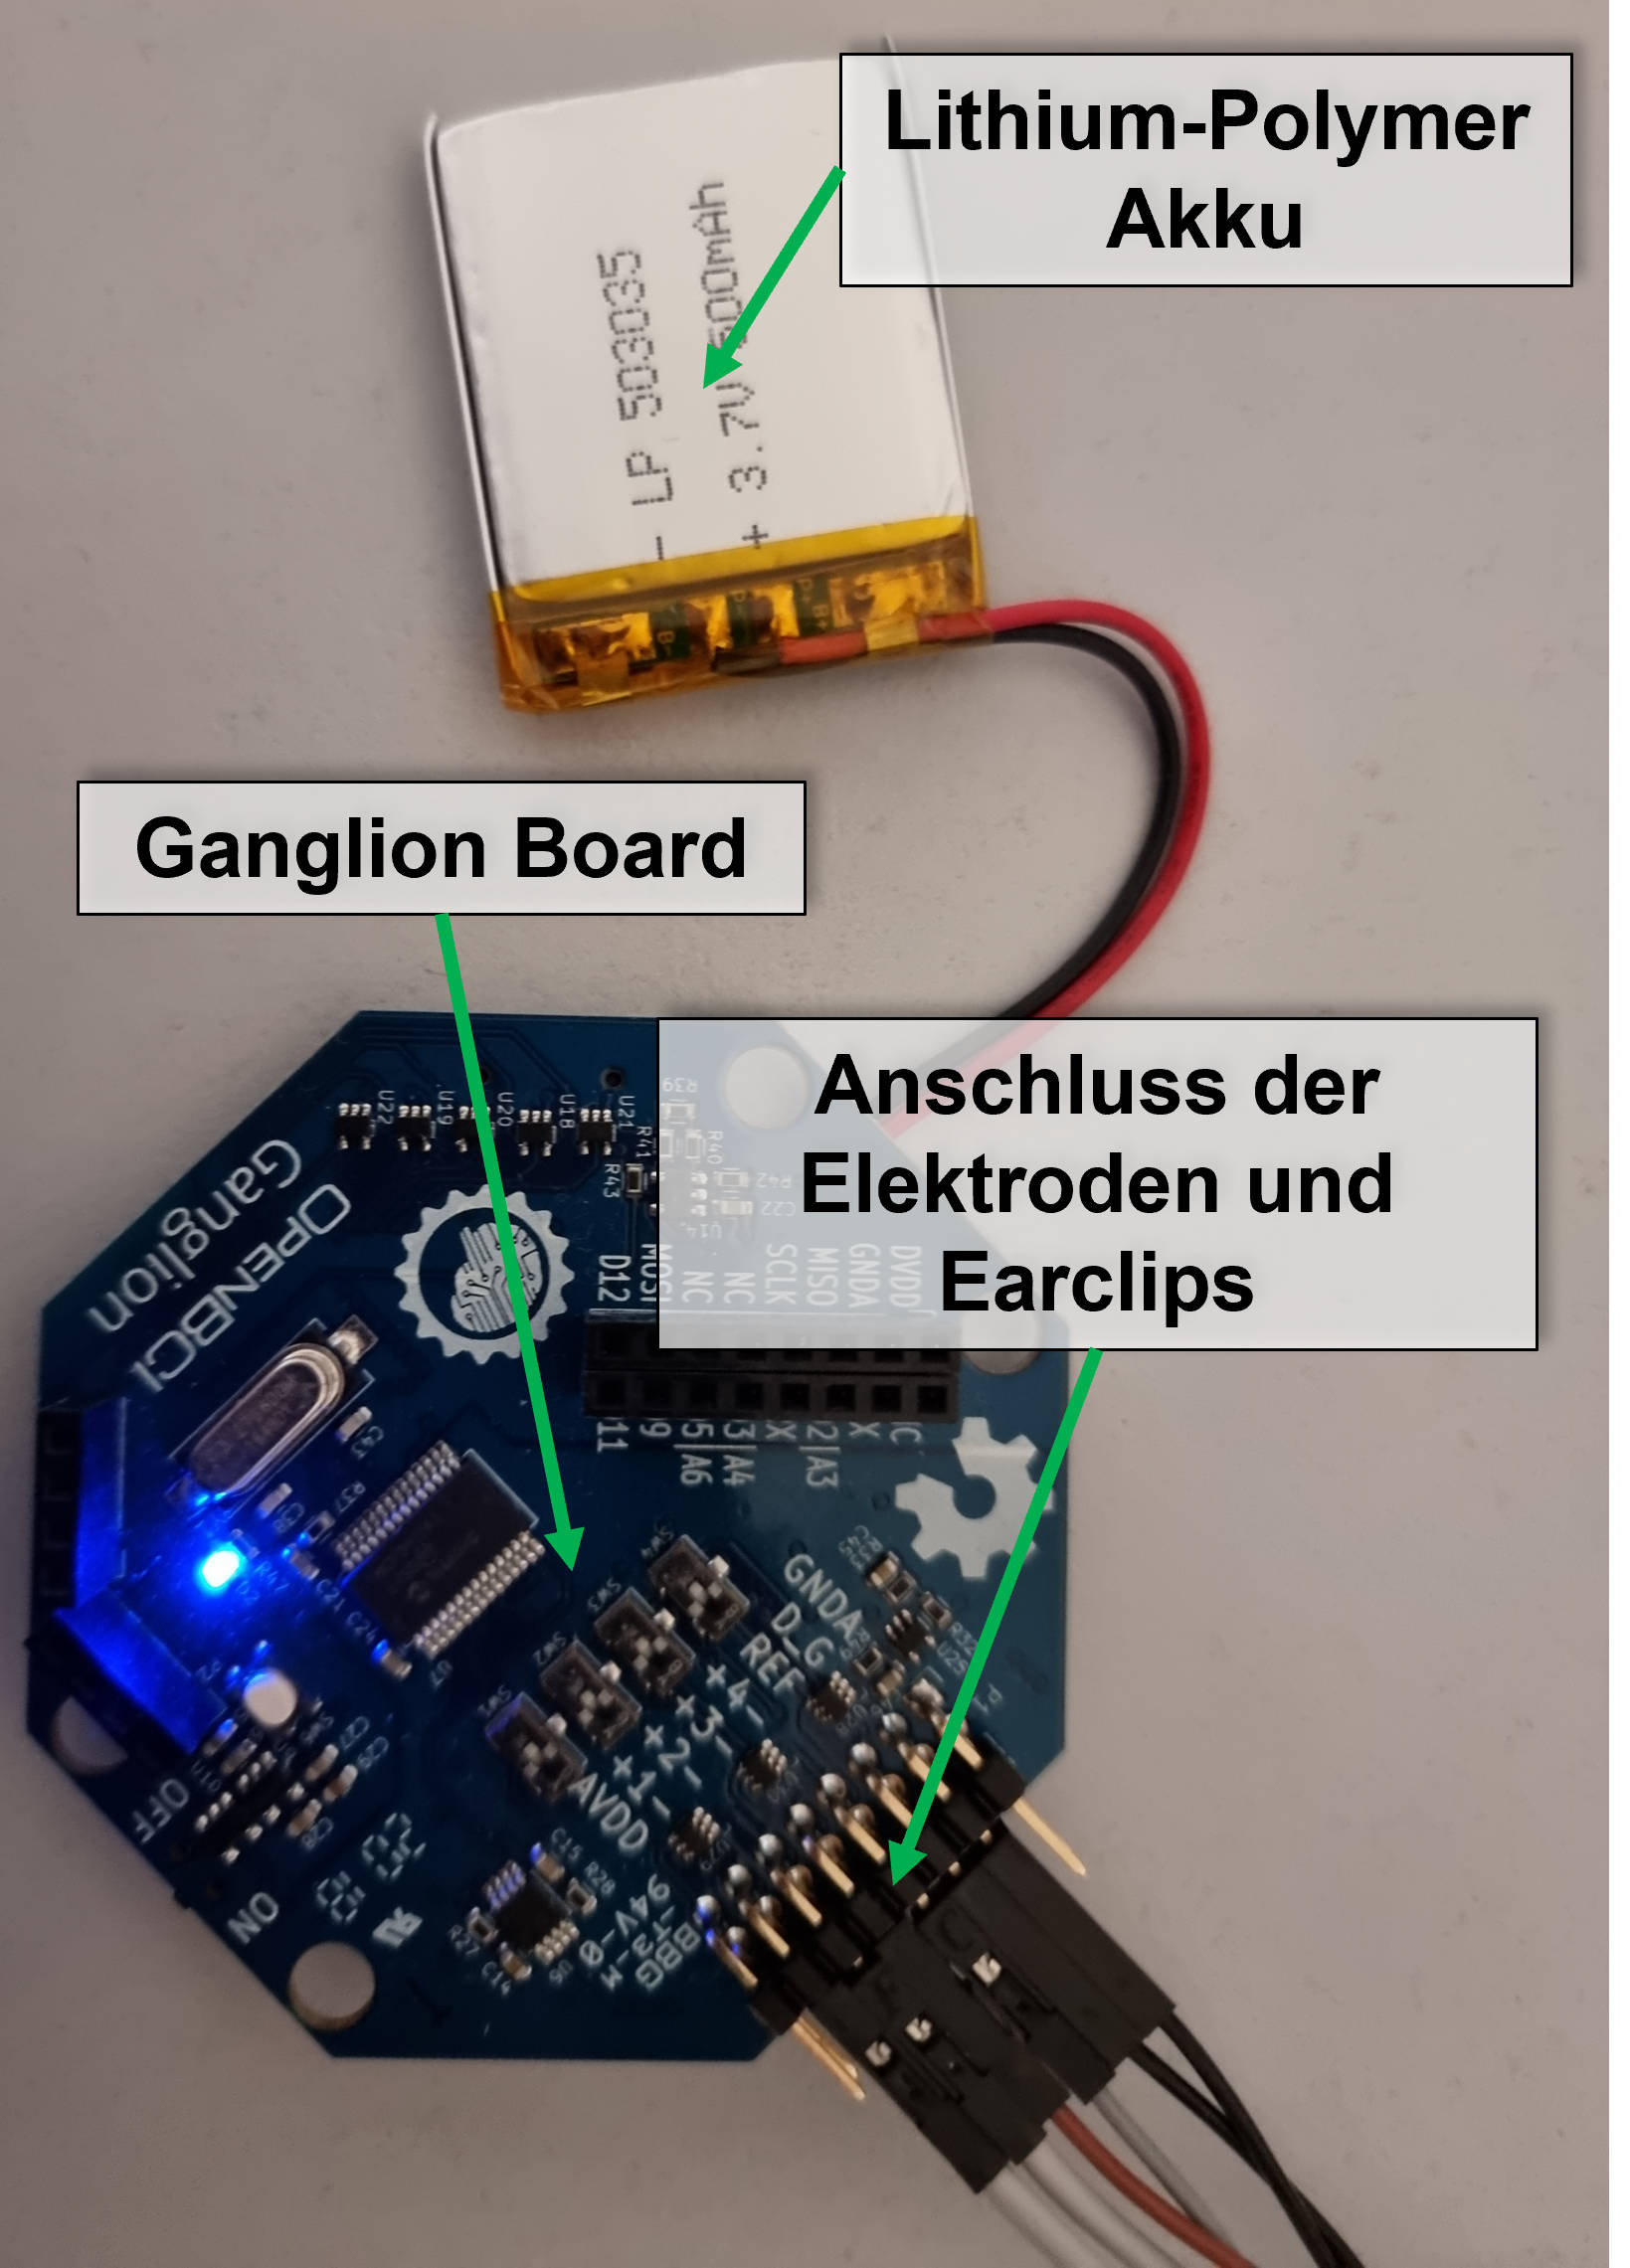
\includegraphics[width=0.3\textwidth]{pictures/Ganglion-Board-annotated.png}
%     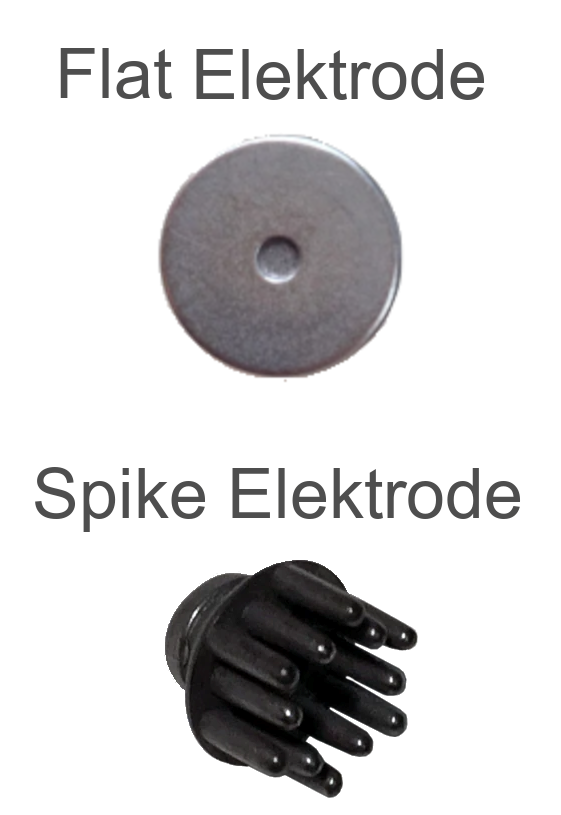
\includegraphics[width=0.15\textwidth]{pictures/spike_flat_elektroden.png}
%     \caption{Das EEG und Zubehör. Links sieht man die typische Anwendung des EEG im Versuchsaufbau. In der Mitte ist das Ganglion Board genauer dargestellt. Rechts sind eine flache Elektrode und eine Spike-Elektrode zu sehen.}
%     \label{EEG-Zubehor}
% \end{figure}

% Als EEG haben wir letztes Jahr das Ganglion Board von OpenBCI verwendet.
% Dieses bietet vier Kanäle, heißt vier Elektroden für die Kopfhaut, sowie eine Referenz- und eine Erdungselektrode. % TODO: Erdungselektrode: Was und wieso?

% Doch obwohl dieses gut funktioniert hat, hat es ein großes Problem: Es kostet ca. \SI{500}{\eur}.
% Dies ist zwar günstig verglichen mit einigen Alternativen, vor allem medizinisch zugelassenen. 
% Für uns ist es jedoch immer noch zu teuer, um unser Ziel zu erfüllen, auch Privatpersonen, vor allem Anfänger, zu interssieren.

% Deswegen wollen wir unser eigenes EEG entwickeln und bauen, mit dem Ziel eine kostengünstigere sowie flexiblere Alternative zu den auf dem Markt angebotenen Modulen qualitativ zu erproben.
% Unser EEG von OpenBCI werden wir also weiter verwenden, sodass wir es mit unserem eigenen EEG vergleichen können. 

% Während wir das EEG entwickelten, wollten wir außerdem bereits mit dem Entiwickeln und Testen einer KI beginnen.
% Dazu haben wir einen Datensatz im Internet gefunden, in welchem der Ersteller mit seinem eigenen 16-Kanal EEG von OpenBCI Daten aufgenommen hat.
% Er hatte das Ziel, 
% Dabei hat er entweder links, rechts oder nicht gedacht und währenddessen EEG-Daten aufgenommen.
% Im folgenden Abschnitt wird nun beschrieben wie wir dabei schrittweise vorgegangen sind.

\subsubsection{Bau unseres eigenen EEG}
 
% Ein EEG stellt vereinfacht nur ein sehr präzises Spannungsmessgerät dar, welches Potentialdifferenzen (Spannungen) im $\mu V$-Bereich messen und anzeigen kann. 
Die Spannungen, die von den Neuronen durch den Schädel dringen, sind zu gering (unterhalb von einigen hundert Mikrovolt), um direkt von einer Messeinheit verarbeitet werden zu können, es muss zunächst eine Verstärkung des aufzuzeichnenden Signals erfolgen. \cite{EEGHausarbeit}
% Die für EEG-Messungen relevante Spannungen liegen meist im Bereich von einigen hundert Mikrovolt. 

Ebenfalls müssen die gewünschten Frequenzen vorab mittels aktiver Filter herausgefiltert werden, um später eine genaue Signalanalyse zu ermöglichen. 
Je nachdem, was für Phänomene genau untersucht werden sollen, können entsprechend unterschiedliche Frequenzbereiche herausgefiltert werden. 
Beispielsweise liegen Alpha-Wellen, die ein bestimmtes Signalschema darstellen und eine wichtige Rolle bei der Konzentration sowie visuellen Verarbeitung spielen, in einem Frequenzbereich von 8 bis 13 Hz. \cite{Praktikum, Birbaumer2010, wiki:Berger-Effekt}
 
 Darüber hinaus wird eine Einheit benötigt, die das Ausgangssignal misst und aufzeichnet, damit es weiterverarbeitet und analysiert werden kann. 
 
Sowohl für die Filterung als auch für die Verstärkung werden sogenannte Operationsverstärker (OPV) verwendet. 
In Abb. \ref{fig:OPV} sieht man rechts das Schaltzeichen mit den jeweiligen Anschlüssen und links einen OPV in einem DIL-Gehäuse. 
 
 \begin{figure}[h!]
    \centering
    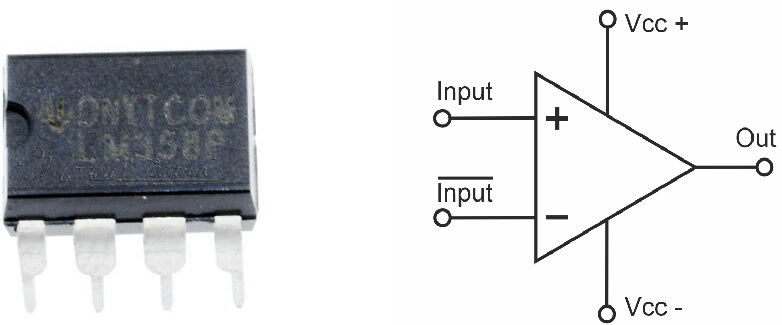
\includegraphics[width=0.5\linewidth]{pictures/OPV_cropped.png}
    \caption{Links: 2-fach OPV LM358 in einem DIL-Gehäuse, Rechts: OPV als Schaltbild }
    \label{fig:OPV}
\end{figure}

OPVs finden vor allem in der Mess- und Regeltechnik Anwendung und bestehen aus Transistoren, die zu integrierten Schaltkreisen zusammengefügt werden.
Dabei lässt sich die interne Schaltung eines OPVs allgemein in zwei Schaltungensteile untergliedern, den sog. Differenzverstärker, der später für die Potentialmessung wichtig wird, und die dahinter geschaltete Gegentaktendstufe, welche
für die Leistungsverstärkung zuständig ist.
Ihr geringer Ausgangswiderstand sowie der hohe Eingangswiderstand als auch der hohe Spannungsverstärkungsfaktor, machen den OPV passend für die Anwendung als EEG-Verstärker.

OPVs besitzen, neben den Anschlüssen für die Stromversorgung, drei für ihre Funktion wichtige Anschlüsse, einen invertierenden und einen nicht-invertierenden Eingang sowie einen Ausgang, über welche er angesteuert werden kann.

Legt man nun über beiden Eingängen jeweils unterschiedliche Spannungen $U_{1}$ und $U_{2}$ an, so wird am Ausgang des OPVs die Differenz der beiden Spannungen ausgegeben. Also gilt: $U_{2} - U_{1} = U_{\textrm{Diff}}$. 
Dies macht man sich nun zu Nutze, um die Spannungen bzw. Potentialdifferenzen zwischen zwei Elektroden zu messen. 
% Wie oben bereits beschrieben wird dabei immer die Potentialdifferenz zwischen einer Elektrode, die sich auf der Kopfhaut und einer Referenzelektrode, die sich am Ohrläppchen befindent, gemessen. 

Zudem lassen sich mit einem OPV und wenigen weiteren Bauteilen einfach aktive Filter bauen.

Die Grundschaltung für unsere EEG beruht auf einem englischsprachigem Internetartikel, in dem eine Verstärkerschaltung für ein EEG beschrieben war. Die von uns angepasste Schaltung ist in Abb. x zu sehen.
Diese mussten wir aber etwas verändern, um den gewünschten Frequenzbereich herauszufiltern.
Basis dieser Schaltung bildet der Instrumentenverstärker AD620AN, welcher extra für EEG- und EKG-Anwendungen entwickelt wurde.

\begin{figure}
    \centering  
    \begin{circuitikz}[european, scale=0.4, transform shape]
        \draw (0,0) node[dipchip, num pins=8, no topmark, external pins width=0.0] (C) {AD620};
        % Verbinde Pins 1 und 8 über Widerstand
        \draw 
            (C.pin 1) -- ++ (-0.5,0) 
            to ++(0,1) 
            to [R,R={\SI{560}{Ω}}] ++(2.7,0) 
            to ++(0,-1) 
            to (C.pin 8);
        % Inputs
        \node[left=1.5 of C.pin 2, iecsocketR] (inputNeg) {};
        \node[left=1.5 of C.pin 3, iecsocketR] (inputPos) {};
        \node[above=0cm of inputNeg, xshift=2em, yshift=-1ex] {\small Input $+$};
        \node[above=0cm of inputPos, xshift=2em, yshift=-1ex] {\small Input $-$};
        \draw
            (C.pin 2) to (inputNeg.east)
            (C.pin 3) to (inputPos.east);
        \draw
            (C.pin 7) to  ++ (1.5,0) to ++ (0,0.75) node[vcc]{\SI{9}{\volt}}
            (C.pin 4) to ++ (-1,0) node[vee]{\SI{-9}{\volt}};
        \node[op amp, right=6 of C, yshift=0.21cm] (opamp1) {};

        % \node at ($(C.pin 6) + (2,0)$) (foo) {};
        % \draw (C.pin 6) to (foo);
        % \draw (foo) to [R={\SI{318}{kΩ}}, -*] ++(2, 0);
        \draw (C.pin 6) to ++(2,0);
        \draw 
            (opamp1.+) node[left] {}
            (opamp1.-) node[left] {}
            (opamp1.out) node[right] {}
            (opamp1.up) -- ++(0,1.5) node[vcc]{\SI{9}{\volt}}
            (opamp1.down) -- ++(0,-1.5) node[vee]{\SI{-9}{\volt}}
            (opamp1.+) to [R={\SI{318}{kΩ}}, -*] 
            ++(-2,0) to [R={\SI{318}{kΩ}}, -*] 
            ++(-2,0) to ++(0,-1.5)
            to [C,l_={\SI{10}{\nano\farad}}, -*] ++(1.25,0)
            to [C,l_={\SI{10}{\nano\farad}}] ++(2.5,0)
            to[short,-*] ++(0,1.5)
            (4.84,-0.3) to (4.84,-4) 
            to [C,l={\SI{20}{\nano\farad}}] ++(0,-2) node[rground]{}
            % (C.pin 6) to ++(2,0)
            (4.1,-1.8) to (4.1,-2.5) to [R,l_={\SI{158}{kΩ}}] ++(0,-2) to ++(0,-1.5) node[rground]{} 
            (opamp1.-) to ++(-1,0) to ++(0,1) to ++(3.5,0) to[short,-*] ++(0,-1.5)
            (opamp1.out) to [C={\SI{220}{\nano\farad}},-*] ++(2,0) to [C={\SI{220}{\nano\farad}}] ++(2,0)
            (11.23,0.25) to [R={\SI{47}{kΩ}}] ++(0,-4) node[rground]{} 
            (11.23,0.25) to [C, l={\SI{220}{\nano\farad}}] ++(0,3) to [short,-*] ++(2,0) to [R, l_={\SI{220}{kΩ}},-*] ++(0,-3.05);
            
        \node[op amp, right=4 of opamp1,yshift=-0.49cm] (opamp2) {};
        \draw 
            (opamp2.+) node[left] {}
            (opamp2.-) node[left] {}
            (opamp2.out) node[right] {}
            (opamp2.up) -- ++(0,1.5) node[vcc]{\SI{9}{\volt}}
            (opamp2.down) -- ++(0,-1.5) node[vee]{\SI{-9}{\volt}}
            (opamp2.out) to[short,*-] ++(0,3.525) to ++(-2.4,0)
            (opamp2.+) to ++(-0.5,0) to ++(0,-3) node[rground]{}
            (15.6,-0.27) to [R, l={\SI{180}{kΩ}},-*] (17.6,-0.27)
            (17.6,-0.27) to[C, l_={\SI{100}{\nano\farad}}] ++(0,-3.5) node[rground]{}
            (17.6,-0.27) to [R, l={\SI{180}{kΩ}}] ++(0,3) to[short, -*] ++(1.9,0) to[C, l_={\SI{25}{\nano\farad}},-*] ++(0,-2.96);
        \node[op amp, right=4 of opamp2,yshift=-0.45cm] (opamp3) {};
        \draw 
            (opamp3.+) node[left] {}
            (opamp3.-) node[left] {}
            (opamp3.out) node[right] {}
            (opamp3.up) -- ++(0,1.5) node[vcc]{\SI{9}{\volt}}
            (opamp3.down) -- ++(0,-1.5) node[vee]{\SI{-9}{\volt}}
            (17.6,-0.27) to[R={\SI{100}{kΩ}}] (opamp3.-)
            (opamp3.+) to ++(-0.5,0) to ++(0,-2.6) node[rground]{}
            (opamp3.out) to [short,*-] ++(0,3.46) to ++(-2.5,0);
        \node[op amp, right=4 of opamp3,yshift=0.48cm] (opamp4) {};
        \draw 
            (opamp4.+) node[left] {}
            (opamp4.-) node[left] {}
            (opamp4.out) node[right] {}
            (opamp4.up) -- ++(0,1.5) node[vcc]{\SI{9}{\volt}}
            (opamp4.down) -- ++(0,-1.5) node[vee]{\SI{-9}{\volt}}
            (opamp3.out) to [big elko, l_={\SI{1}{\mu\farad}}] ++(4,0)
            (opamp4.+) to[R,l_={\SI{1}{MΩ}},*-] ++(0,-3.25) node[rground]{}
            (opamp4.-) to[short,-* ] ++(-1.4,0) to ++(-1,0) to [C, l={\SI{10}{\nano\farad}}] ++(0,3) to [short,-*] ++(1,0) to[R,l={\SI{100}{kΩ}}] ++(0,-3)
            (opamp4.out) to ++(0,3.5) to ++(-3.7,0)
            (24.6,0.5) to (24.6,-2.3) to [R,l_={\SI{220}{Ω}}] ++(0,-2)
            (24.6,-4.3) to [vR, l=\SI{1}{\kohm}, *-] ++(0,-2) node[rground]{}
            (24.6,-4.3) to ++(-0.5,0) to[short,-*] ++(0,-0.74) 
            (opamp4.out) to[big elko, l_={\SI{100}{\mu\farad}},*-o] ++(2,0);
    \end{circuitikz}
    \caption{Schaltplan}
    \label{fig:my_label}
\end{figure}
 
\subsection{Fourier-Analyse}

Die Fourier-Analyse kann die verschiedenen zugrundeliegenden Frequenzen von Datenfolgen, Funktionen, und mehr bestimmen, indem diese in Sinus-Kurven mit verschiedenen Frequenzen zerlegt werden, welche summiert möglichst nah am Ursprung liegen. 
Dafür kriegt jede Frequenz eine Amplitude zugeordnet.
Die Fourier-Analyse dient also zur Spektralanalyse.

Wir nutzen in unserem Projekt die Fast Fourier Transformation (FFT), welche lediglich eine komplexere aber effizientere Form der Diskreten Fourier Transformation (DFT) ist.
% TODO: Beschreibung DFT?

Aus der FFT folgt ein Array (eine Liste) an komplexen Zahlen. 
Der Index eines Wertes in der Liste bestimmt, für welche Frequenz der Wert gilt (erster Wert: 1 Hertz, zweiter Wert: 2 Hertz, etc.). Nun muss für jede komplexe Zahl der Abstand zum Ursprung bestimmt werden, also der absolute Betrag. 
Dieser entspricht dann der Amplitude der Frequenz. So lässt sich bestimmen, welche Frequenzen am stärksten vorkommen. Außerdem können dann Frequenzen herausgefiltert werden, indem die Werte bei den entsprechenden Indices auf 0 gesetzt werden. 

Eine FFT kann Elektroenzephalogramme fast verlustfrei repräsentieren. 
Dies lässt sich erkennen, wenn man mithilfe der durch die FFT entstandenen Spektralanalyse die Daten rekonstruiert (Inverse Fast Fourier Transformation, IFFT). 
Es werden dazu die Sinus-Kurven der Frequenzen mit den entsprechenden Amplituden multipliziert und dann addiert.

Wie in Abb. \ref{fig:ifft} sichtbar, ist diese Rekonstruktion kaum von den originalen Daten unterscheidbar. % TODO: Gesamtdifferent oder anderes mathematische Maß für Ähnlichkeit anstelle / zusätzlich zu graphischem?

\begin{figure}[h!]
    \centering
    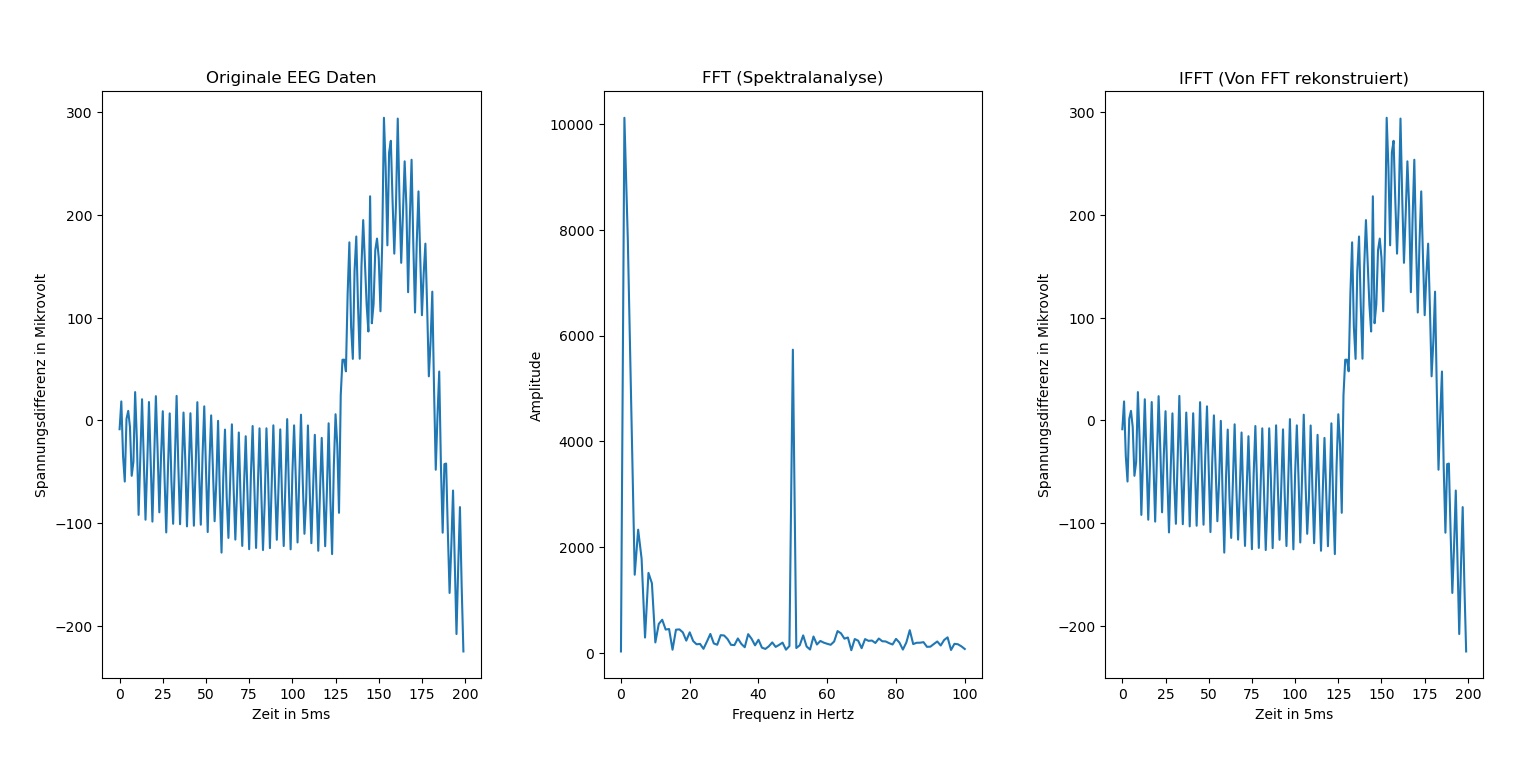
\includegraphics[width=\linewidth]{pictures/blink_fft_ifft.png}
    \caption{Links: Originale EEG Daten, Mitte: Die Amplituden der Frequenzen dieser Daten, Rechts: Die Umkehrung der Frequenzdaten. Da der rechte Graph dem linken sehr ähnlich ist, lässt sich erkennen, dass es bei der Fourier Analyse keinen großen Informationsverlust gibt.}
    \label{fig:ifft}
\end{figure}

\subsection{Neuronales Netz}

Ein neuronales Netzwerk besteht aus drei Teilen: der Eingabeschicht, den verdeckten Schichten und der Ausgabeschicht. 

Die Eingabeschicht ist eine Liste aus Zahlen. 
Sie gibt an, welche Eingaben das Netzwerk bekommen soll, z.B. die Helligkeit der Pixel eines Graustufen-Bildes.

Die verdeckten Schichten sind eine Ansammlung von in mehrere Schichten unterteilten Neuronen.

Jedes Neuron besitzt eine sog. Aktivierung, die meist als Zahl zwischen 0 und 1 oder -1 und 1 angegeben werden kann. 
Die Neuronen verschiedener Schichten sind durch sogenannte Gewichte (\eng{weights}) verbunden, die ebenfalls einen beliebigen Wert haben können.
Die Ausgaben / Vorhersagen des neuronalen Netzwerkes werden von den Aktivierungen der Neuronen in der Ausgabeschicht abgelesen.

Bei neuronalen Netzwerken gibt es zwei relevant Verfahren: Den Forward Pass und die Backpropagation.

Ersteres beschreibt das propagieren von den Eingabewerten durch das Netzwerk.
Zuerst werden die Aktivierungen der Neuronen in der Eingabeschicht gesetzt und danach die Aktivierungen der Neuronen der nächsten Schicht berechnet, welche dann wiederum für der nächsten Schicht verwendet werden und so weiter.
Dadurch werden die Eingaben von Schicht zu Schicht bis zur Ausgabe weiterverarbeitet.
Der Forward Pass ist zur Verwendung eines Netzwerks notwendig.

Er bietet außerdem den ersten Schritt der Backpropagation, die für das Lernen des Netzwerks verantwortlich ist.
Nachdem alle Aktivierungen gesetzt wurden, werden die Aktivierung der letzten Schicht, also die Ausgaben, bewertet.
Wir verwenden Supervised Learning, heißt wir nutzen zur Bewertung Trainingsdaten, die wir vorher \eng{gelabelt}, ihnen also die korrekten Ausgabedaten zugewiesen haben.

Dann wird jedes einzelne Ausgabeneuron \enquote{bewertet}, indem die Differenz zwischen der tatsächlichen Aktivierung nach dem Forward Pass und den zugewiesenen korrekten Ausgaben gebildet wird.

Diese Differenz zwischen ist-Zustand und soll-Zustand wird nun in der Backpropagation verwendet, um die Gewichte zwischen Ausgabe- und vorletzter Schicht anzupassen, denn mit ihm kann der sogenannte delta-Wert eines Neurons bestimmt werden.
Dieser entspricht der Änderung der Aktivierung eines Neurons, die notwendig wäre, damit ein Forward Pass von dort aus ein korrektes Ergebnis liefert.

Auf die Berechnung des delta-Werts werden wir dieses Jahr nicht weiter eingehen, da es für uns nicht direkt relevant ist.
Interessant ist womöglich nur noch, dass dafür die delta-Werte der nächsten Schicht (in Richtung Ausgabe) benötigt werden und daher der \eng{backward} (dt. rückwärts) Teil im Namen kommt.

Mithilfe dieses delta-Werts kann dann auch bestimmt werden, wie die Gewichte angepasst werden müssten, um diese gewünschte Änderung umzusetzen:

\form{\[
	\Delta W_{i,j} = \eta * \delta_i * a_j
\]}

Und entsprechend angepasst werden mit:
\form{\[
    W_{i,j} = W_{i,j} + \Delta W_{i,j}
\]}

\noindent wobei $i$ das Neuron näher zur Ausgabe, $j$ das Neuron näher zur Eingabe und $W_{i,j}$ das Gewicht zwischen diesen beiden ist.

Die Multiplikation mit $a_j$ findet statt, um zu ermöglichen, dass die Änderung der Gewichte entsprechend ihres tatsächlichen Einflusses geschieht, bedeutet, wenn ein Gewicht mit einem Neuron verbunden ist, welches kaum aktiv ist (eine niedrige Aktivierung hat), wird das Gewicht zu diesem auch kaum angepasst, und wenn es negativ ist, dann wird die Änderung umgekehrt, was auch notwendig ist, um das Ziel zu erreichen.

$\eta$ ist die sogenannte Lernrate.
Sie ist meist ein sehr niedriger Wert (0.01, 0.0001, etc.) und ist wichtig für das Kernkonzept des Lernen eines neuronalen Netzwerks:
Sie sorgt dafür, dass bei jedem Trainingsdatensatz die Gewicht nur etwas an diesen angepasst werden, sodass das gesamte Training die Gewichtsanpassungen aller Trainingsdatensätze und somit hoffentlich auch eine Generalisierung dieser darstellt.

Insgesamt lässt sich also sagen, dass ein neuronales Netzwerk versucht, diese Differenz $\textrm{ist} - \textrm{soll}$ zu minimieren.
Diese Differenz ist also ähnlich einer Verlustfunktion und lässt sich tatsächlich auch in einer tatsächlichen Verlustfunktion für Supervised trainierte neuronale Netzwerke, dem Mean Squared Error, wiederfinden:

\form{ \[
	C_0 = (a_0 - y)^2
\]}
\noindent wobei $C_0$ der Verlust der Ausgabeschicht (Schicht $0$, da Indexierung der Schichten bei der Ausgabe beginnt), $a_0$ der Vektor aller Aktivierungen der Ausgabeschicht, und $y$ ein Vektor der richtigen Ausgaben für die Eingaben, mit denen die Aktivierungen berechnet wurden, ist.

Es gibt verschiedene Arten von Schichten in neuronalen Netzwerken; wir verwenden hauptsächlich \feng{Fully Connected} und \feng{Convolutional} Schichten.

\subsubsection{Fully Connected Schichten} 

Bei Fully Connected Schichten sind alle Neuronen eines Layers mit allen Neuronen des nächsten Layers verbunden.
Außerdem hat typischerweise jedes Neuron einen sogenannten Bias, der hinzu addiert wird.

% \threesub{{Forward pass}} \label{forward-prop}

Zur Berechnung der Aktivierungen der Neuronen gibt es den sogenannten \feng{Forward Pass}. 
Dabei beginnt man in der ersten verdeckten Schicht damit, für alle Neuronen die sogenannte Netzeingabe zu berechnen. 
Um die Netzeingabe eines Neurons zu berechnen, werden alle Aktivierungen der vorherigen Schicht mit den von dem Neuron dorthin führenden Gewichten multipliziert und aufsummiert.

Der Bias ist eigentlich auch ein Gewicht, jedoch ist er mit einem Neuron verbunden, das immer die Aktivierung 1 hat. \cite{brotcrunsher:forwardpass}

Die Formel für die Berechnung der Netzeingabe eines Neurons in einer Fully Connected Schicht lautet also:

\form{\[
	\netin_j = \sum_{L} (a_{L} * W_{Lj}) + b_{j}
	\]}
\noindent wobei $\netin_j$ die Netzeingabe des Neurons $j$, $L$ die vorherige Schicht, $a_L$ der Vektor aller Aktivierungen der Schicht $L$, $W_{Lj}$ der Vektor aller Gewichte zwischen dem Neuron $j$ und den Neuronen der Schicht $L$, und $b_j$ der Bias des Neurons $j$ ist. 

% \begin{figure}
%     \def\layersep{3cm}
%     \centering
%     % \begin{minipage}[t]{0.6\linewidth}\vspace{0pt}%
%     \begin{tikzpicture}[
%         scale=1.2,
%         shorten >=1pt,->,draw=black!70, node distance=\layersep,
%         neuron/.style={circle,fill=black!25,minimum size=20,inner sep=0},
%         edge/.style 2 args={pos={(mod(#1+#2,2)+1)*0.33}, font=\tiny},
%         distro/.style 2 args={
%             edge={#1}{#2}, node contents={}, minimum size=0.6cm, path picture={\draw[double=orange,white,thick,double distance=1pt,shorten >=0pt] plot[variable=\t,domain=-1:1,samples=51] ({\t},{0.2*exp(-100*(\t-0.05*(#1-1))^2 - 3*\t*#2))});}
%           },
%         weight/.style 2 args={
%             edge={#1}{#2}, node contents={\pgfmathparse{0.35*#1-#2*0.15}\pgfmathprintnumber[fixed]{\pgfmathresult}}, fill=white, inner sep=2pt
%           }
%       ]
%     % Input layer
%     \foreach \y in {1,...,2}
%         \node[neuron, fill=green!40] (i\y) at (0,\y+1) {$i_\y$};
%     \node[neuron, fill=orange!40] (b1) at (0, 4.5) {$b_1$};
%     % Hidden layer
%     \foreach \y in {1,...,4}
%         \path node[neuron, fill=blue!40] (h\y) at (\layersep,\y) {$h_\y$};
%     \node[neuron, fill=orange!40] (b2) at (\layersep, 5.5) {$b_2$};
%     % Output node
%     \node[neuron, fill=red!40] (o) at (2*\layersep,2.5) {$O$};
    
%     % Connect every node in the input layer with every node in the hidden layer.
%     \foreach \source in {1,...,2}
%         \foreach \dest in {1,...,4}
%             \path (i\source) edge (h\dest);
%     % Connect bias in the input layer with every node in the hidden layer.
%     \foreach \dest in {1,...,4}
%         \path[red!20] (b1) edge (h\dest);
%     % Connect every node in the hidden layer with the output layer
%     \foreach \source in {1,...,4}
%         \path (h\source) edge (o);
%     % Connect bias in the hidden layer with the output layer
%     \path[red!20] (b2) edge (o);
        
%     % Draw weights for all regular edges.
%     \foreach \i in {1,...,2}
%     \foreach \j in {1,...,4}
%     \path (i\i) -- (h\j) node[weight={\i}{\j}];
%     \foreach \i in {1,...,4}
%     \path (h\i) -- (o) node[weight={\i}{1}];
%     % Draw weights for bias edges.
%     \foreach \j in {1,...,4}
%     \path (b1) -- (h\j) node[weight={3}{\j}];
%     \path (b2) -- (o) node[weight={5}{1}];
%     \end{tikzpicture}
%     % \end{minipage}

    
%     % \begin{minipage}[t]{0.5\linewidth}\vspace{0pt}%
%     % \begin{alignat*}{2}
%     %     &h_4 = i_2 * 0.1 + i_1 * (-0.25) \\
%     %     &h_3 = i_2 * 0.25 + i_1 * (-0.1) \\
%     %     & ... \\
%     %     & O = h_4 * 1.25 + h_3 * 0.9 + h_2 * 0.55 + h_1 * 0.2 \\
%     % \end{alignat*}
%     % \end{minipage}
%     \caption{Caption}
%     \label{fig:dense_nn}
% \end{figure}

Um aus dieser Netzeingabe nun die Aktivierung zu berechnen, benötigt man eine Aktivierungsfunktion, die zum einen dafür sorgt, dass die Aktivierung begrenzt und somit ein unendliches Wachstum der Aktivierungen und entsprechend Gewichte verhindert wird, und zum anderen sicherstellt, dass es keine Linearität zwischen Eingaben und Ausgaben gibt. 
Dadurch kann das Netzwerk vor allem Klassifizierungsaufgaben besser erlernen. % TODO: Quelle

\begin{figure}[h!]
    \centering
    \begin{minipage}[t]{0.5\linewidth}\vspace{0pt}%
        \begin{tikzpicture}
        \begin{axis}[
            xlabel={Netzeingabe}, ylabel={Aktivierung}, domain={-10:10}, samples=100,
            no markers, legend pos=south east
        ]
            \addplot {1 / (1 + 2.71828^(-x))};
            \addplot{tanh(x)};
            \legend{$\sig(x)$, $\tanh(x)$};
        \end{axis}
        \end{tikzpicture}
        \caption{Aktivierungsfunktionen im Vergleich}
        \label{fig:act_funcs}
    \end{minipage}
\end{figure}

Letztes Jahr haben wir die Sigmoid-Funktion genutzt, welche sicherstellt, dass der Eingabewert immer zwischen 0 und 1 liegt (s. Abb. \ref{fig:act_funcs}.

\[
    \sig(x) = \frac{1}{1+e^{-x}}
\]

Doch dieses Jahr setzen wir auf die $\tanh$-Aktivierungsfunktion, bei der die Werte immer zwischen -1 und 1 liegen (s. Abb. \ref{fig:act_funcs}.
Mit der Sigmoid-Aktivierungsfunktion war aufgrund der Beschränkung auf positive Zahlen das Abziehen von der Aktivierung eines Neurons durch ein vorhergehendes nicht möglich und somit die Komplexität und Möglichkeiten eines neuronalen Netzwerkes eingeschränkt.

Dieses Verfahren zur Berechnung der Aktivierung wird dann für jedes Neuron in jeder Schicht wiederholt.
Da aber immer die Aktivierungen der vorherigen Schicht ($a_{L}$) benötigt, muss dieser Prozess von der Eingabeschicht aus zur Ausgabeschicht hin durchgeführt werden, daher auch der Name \feng{Forward Pass}.

Fully Connected Schichten sind die \enquote{Standard}-Schicht bei neuronalen Netzwerken. 
Sie können und werden vielseitig eingesetzt, doch haben den Nachteil, dass sie \enquote{global} sind, d.h. sie 

\subsubsection{Convolutional Layer}

Im Gegensatz zu den den fully-connected Schichten, in denen jedes Neuron einer Schicht mit allen Neuronen der nächsten Schicht verbunden ist, sind die Neuronen der Convolutional Layer jeweils nur mit ein paar Neuronen der nächsten Schicht verbunden.
Convolutional Layer nutzen einen sogenannten Filterkernel, um die Aktivierungen der Neuronen der nächsten Schicht zu bestimmen.
Der Filterkernel ist eine Liste an Zahlen, hat immer genauso viele Dimensionen wie die Eingaben und ist generell kleiner als sie. 

Um die Werte der nächsten Schicht zu bestimmen, \enquote{wandert} der Filterkernel über die Eingaben, sodass er jede mögliche Position einmal einnimmt.
Bei jedem Schritt wird der Filterkernel \enquote{angwendet}, indem das Skalarprodukt des aktuellen Ausschnittes der Eingaben und des Filters berechnet wird. 
Um das Skalarprodukt zu berechnen, muss das erste Element des Filterkernels mit dem ersten Element des Eingabenausschnitts, das zweite Element des Flterkernels mit dem zweiten Element des Eingabenausschnittes usw. multipliziert werden und anschließend die Summe von all diesen ausgerechnet werden.
Diese Summen bilden dann die Werte für die nächste Schicht des neuronalen Netzwerkes.
% Die Ausgabe hat also ohne zusätzliches \feng{Padding} (dt. Polsterung) immer die gleiche Dimensionen wie die Eingabe, jedoch in jeder Dimension um zwei verkleinert, da der Kernel 

Beim Trainieren des neuronalen Netzwerkes werden bei Convolutional Layern dann die einzelnen Werte der Kernel als anzupassende Gewichte behandelt.

Der Vorteil von Convolutional Layern ist, dass sie lokal und nicht global arbeiten.
Damit ist gemeint, dass eine normale Fully Connected Schicht ein erwartete Muster nur erkennt, wenn es an seiner Position so auch schon in den Trainingsdaten vorkam.
Da der Kernel jedoch über die Eingaben wandert und alle möglichen Positionen annimmt, kann ein trainierter Kernel das antrainierte Muster überall erkennen, egal, wo es vorkommt.
Deswegen werden Convolutional Schichten sehr gerne bei Bild- und Videoverarbeitung genutzt, wo z.B. zu erkennende Hunde nicht immer auf der gleichen Stelle im Bild sind.

\begin{figure}[h!]
    \centering
    % source: https://tikz.net/conv2d/
    % Convolution operator.
    % Adapted from https://github.com/PetarV-/TikZ/tree/master/2D%20Convolution
    \begin{tikzpicture}[
        2d-arr/.style={matrix of nodes, row sep=-\pgflinewidth, column sep=-\pgflinewidth, nodes={draw}}
      ]
      %TODO: make "unknown" numbers (after current kernel position) empty or "?" ?
      \matrix (mtr) [2d-arr] {
      0 & 1 & 1 & |[fill=orange!30]| 1 & |[fill=orange!30]| 0 & |[fill=orange!30]| 0 & 0 & \\
      };
      \node[left=1.5cm of mtr-1-4] (left-desc) {Eingabe $I$};
      \node[below=0.2em of mtr] (str) {$*$};
      \matrix (K) [2d-arr, below=0.2em of str, nodes={draw, fill=teal!30}] {
        1 & 1 & 0 \\
      };
      \node[left=1.5cm of K-1-2] {Kernel $K$};
      \node[below=0.2em of K] (eq) {$=$};
      \matrix (ret) [2d-arr, below=0.2em of eq] {
      1 & 2 & 2 & |[fill=blue!80!black!30]| 1 & ? & \\
      };
      \node[left=1.5cm of ret-1-3] {Ausgabe ${I * K}$};
    
      \draw[dashed, teal] (mtr-1-4.south west) -- (K-1-1.north west);
      \draw[dashed, teal] (mtr-1-6.south east) -- (K-1-3.north east);
    
      \draw[dashed, blue!80!black] (K-1-1.south west) -- (ret-1-4.north west);
      \draw[dashed, blue!80!black] (K-1-3.south east) -- (ret-1-4.north east);

      \node[above=0.8cm of {$(left-desc) !.5! (mtr-1-4)$},font=\large] {\textbf{1-dimensional}};
      \node[font=\tiny, scale=0.6, shift={(-1.2ex,-2ex)}] at (mtr-1-4) {$\times 1$};
      \node[font=\tiny, scale=0.6, shift={(-1.2ex,-2ex)}] at (mtr-1-5) {$\times 1$};
      \node[font=\tiny, scale=0.6, shift={(-1.2ex,-2ex)}] at (mtr-1-6) {$\times 0$};
      % \foreach \i in {1} {
      %     \foreach \j in {4,5,6} {
      %         \node[font=\small, scale=0.6, shift={(-1.2ex,-2ex)}] at (mtr-\i-\j) {$\times \pgfmathparse{int(mod(\i+\j,2))}\pgfmathresult$};
      %       }
      %   }
    % \end{tikzpicture}
    % \begin{tikzpicture}[
      %   2d-arr/.style={matrix of nodes, row sep=-\pgflinewidth, column sep=-\pgflinewidth, nodes={draw}}
      % ]
      \matrix (mtr2) [2d-arr, right = 2cm of K-1-3] {
      0 & 1 & 1 & |[fill=orange!30]| 1 & |[fill=orange!30]| 0 & |[fill=orange!30]| 0 & 0\\
      0 & 0 & 1 & |[fill=orange!30]| 1 & |[fill=orange!30]| 1 & |[fill=orange!30]| 0 & 0\\
      0 & 0 & 0 & |[fill=orange!30]| 1 & |[fill=orange!30]| 1 & |[fill=orange!30]| 1 & 0\\
      0 & 0 & 0 & 1 & 1 & 0 & 0\\
      0 & 0 & 1 & 1 & 0 & 0 & 0\\
      0 & 1 & 1 & 0 & 0 & 0 & 0\\
      1 & 1 & 0 & 0 & 0 & 0 & 0\\
      };
      \node[below=of mtr2-5-4] {Eingabe $ I$};
      \node[right=0.2em of mtr2] (str) {$*$};
      \matrix (K2) [2d-arr, right=0.2em of str, nodes={draw, fill=teal!30}] {
        1 & 0 & 1 \\
        0 & 1 & 0 \\
        1 & 0 & 1 \\
      };
      \node[below=of K2-3-2] {Kernel $  K$};
      \node[right=0.2em of K2] (eq) {$=$};
      \matrix (ret2) [2d-arr, right=0.2em of eq] {
      1 & 4 & 3 & |[fill=blue!80!black!30]| 4 & ? \\%1\\
      ? & ? & ? & ? & ? \\
      ? & ? & ? & ? & ? \\
      ? & ? & ? & ? & ? \\
      ? & ? & ? & ? & ? \\
      % 1 & 2 & 4 & 3 & 3\\
      % 1 & 2 & 3 & 4 & 1\\
      % 1 & 3 & 3 & 1 & 1\\
      % 3 & 3 & 1 & 1 & 0\\
      };
      \node[below=of ret2-4-3] {Ausgabe ${I * K}$};
    
      \draw[dashed, teal] (mtr2-1-6.north east) -- (K2-1-1.north west);
      \draw[dashed, teal] (mtr2-3-6.south east) -- (K2-3-1.south west);
    
      \draw[dashed, blue!80!black] (K2-1-3.north east) -- (ret2-1-4.north west);
      \draw[dashed, blue!80!black] (K2-3-3.south east) -- (ret2-1-4.south west);

      \node[above=0.8cm of {$(mtr2-1-1) !.5! (ret2-1-5)$},font=\large] {\textbf{2-dimensional}};
    
      \foreach \i in {1,2,3} {
          \foreach \j in {4,5,6} {
              \node[font=\tiny, scale=0.6, shift={(-1.2ex,-2ex)}] at (mtr2-\i-\j) {$\times \pgfmathparse{int(mod(\i+\j,2))}\pgfmathresult$};
            }
        }
    \end{tikzpicture}
    \caption{Eine 1-dimensionale und eine 2-dimensionale Convolutional Schicht. Die farbig hervorgehobenen Felder stellen einen Schritt des Kernels dar; als nächstes würde er ein Feld weiter nach rechts rücken und die Ausgabe auch.} %TODO ?
    \label{fig:conv_layers}
\end{figure}

% \begin{figure}[h!]
%     \centering
%     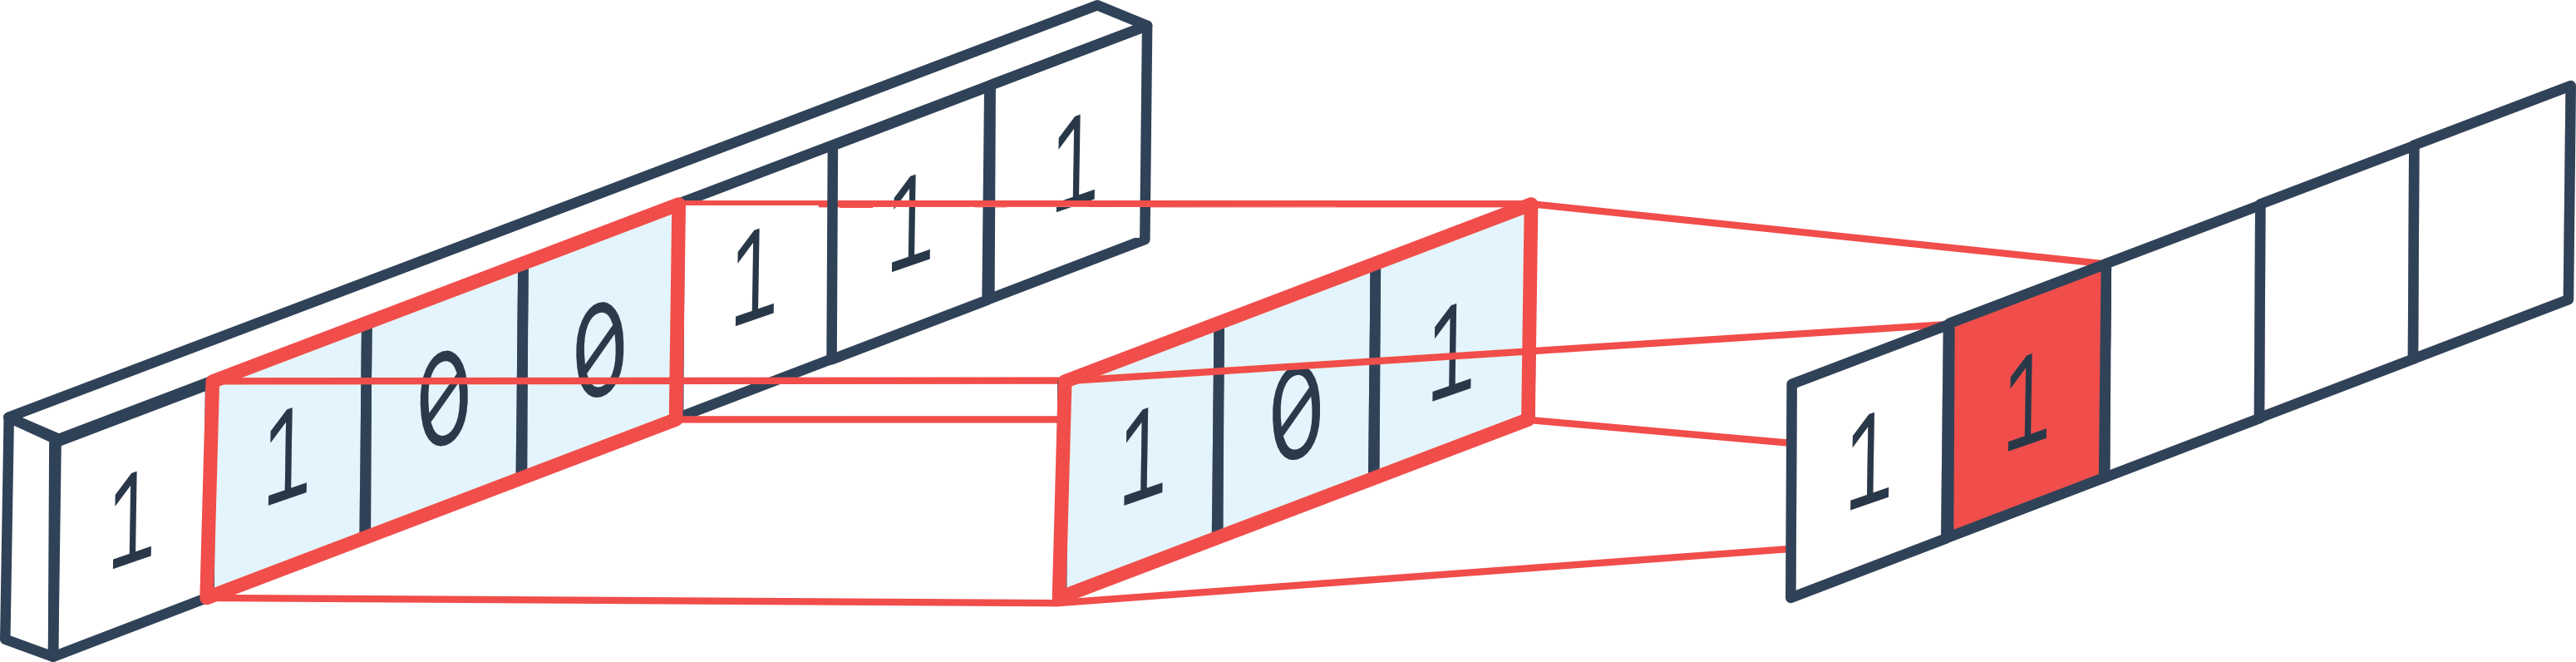
\includegraphics[width=\textwidth]{pictures/1DConv.png}
%     \caption{Darstellung eines Convolutional Layers.}
%     \label{Conv Layer 1}
% \end{figure}

\begin{figure}[h!]
    \centering
    % source: https://tikz.net/conv2d/
    % Convolution operator.
    % Adapted from https://github.com/PetarV-/TikZ/tree/master/2D%20Convolution
    \begin{tikzpicture}[
        2d-arr/.style={matrix of nodes, row sep=-\pgflinewidth, column sep=-\pgflinewidth, nodes={draw}}
      ]
      \matrix (mtr) [2d-arr, right = 2cm of K-1-3] {
      0 & 1 & 1 & |[fill=orange!30]| 1 & |[fill=orange!30]| 0 & |[fill=orange!30]| 0 & 0\\
      0 & 0 & 1 & |[fill=orange!30]| 1 & |[fill=orange!30]| 1 & |[fill=orange!30]| 0 & 0\\
      0 & 0 & 0 & |[fill=orange!30]| 1 & |[fill=orange!30]| 1 & |[fill=orange!30]| 1 & 0\\
      0 & 0 & 0 & 1 & 1 & 0 & 0\\
      0 & 0 & 1 & 1 & 0 & 0 & 0\\
      0 & 1 & 1 & 0 & 0 & 0 & 0\\
      1 & 1 & 0 & 0 & 0 & 0 & 0\\
      };
      \node[below=0cm of mtr] {Eingabe $ I$};
      \node[right=1em of mtr] (str) {$\Large{*}$};
      \matrix (K1) [2d-arr, right=1em of str, yshift=1.5cm, nodes={draw, fill=teal!30}] {
        1 & 0 & 1 \\
        0 & 1 & 0 \\
        1 & 0 & 1 \\
      };
      \matrix (K2) [2d-arr, right=1em of str, yshift=-1.5cm, nodes={draw, fill=violet!30}] {
        0 & 1 & 0 \\
        1 & 0 & 1 \\
        0 & 1 & 0 \\
      };
      \node[above=0cm of K1] {Kernel $K_1$};
      \node[below=0cm of K2] {Kernel $K_2$};
      
      \node (eq) at ($(K1) !.5! (K2) + (K1) !.5! (K2) - (str)$) {$=$};
      
      \matrix (ret1) [2d-arr, right=1em of eq, yshift=1.5cm] {
      1 & 4 & 3 & |[fill=blue!80!black!30]| 4 & ? \\%1\\
      ? & ? & ? & ? & ? \\
      ? & ? & ? & ? & ? \\
      ? & ? & ? & ? & ? \\
      ? & ? & ? & ? & ? \\
      % 1 & 2 & 4 & 3 & 3\\
      % 1 & 2 & 3 & 4 & 1\\
      % 1 & 3 & 3 & 1 & 1\\
      % 3 & 3 & 1 & 1 & 0\\
      };
      \matrix (ret2) [2d-arr, right=1em of eq, yshift=-1.5cm] {
      2 & 2 & 4 & |[fill=blue!80!black!30]| 2 & ? \\%1\\
      ? & ? & ? & ? & ? \\
      ? & ? & ? & ? & ? \\
      ? & ? & ? & ? & ? \\
      ? & ? & ? & ? & ? \\
      % 1 & 2 & 4 & 3 & 3\\
      % 1 & 2 & 3 & 4 & 1\\
      % 1 & 3 & 3 & 1 & 1\\
      % 3 & 3 & 1 & 1 & 0\\
      };
      \node[above=0cm of ret1] {Ausgabe ${I * K_1}$};
      \node[below=0cm of ret2] {Ausgabe ${I * K_2}$};

      % https://latexdraw.com/how-to-draw-curly-braces-in-tikz/
      \draw[decorate, decoration = {brace, amplitude = 10pt, raise = 10pt}] ($(ret1-1-5.north east) + (0, 0.2)$) -- ($(ret1-5-5.south east) - (0, 0.2)$)
      node[pos=0.5,right=20pt,black]{Kanal 1};
      \draw[decorate, decoration = {brace, amplitude = 10pt, raise = 10pt}] ($(ret2-1-5.north east) + (0, 0.2)$) -- ($(ret2-5-5.south east) - (0, 0.2)$)
      node[pos=0.5,right=20pt,black]{Kanal 2};
      
      \draw[dashed, teal] (mtr-1-6.north east) -- (K1-1-1.north west);
      \draw[dashed, teal] (mtr-3-6.south east) -- (K1-3-1.south west);
      
      \draw[dashed, violet] (mtr-1-6.north east) -- (K2-1-1.north west);
      \draw[dashed, violet] (mtr-3-6.south east) -- (K2-3-1.south west);
    
      \draw[dashed, blue!80!black] (K1-1-3.north east) -- (ret1-1-4.north west);
      \draw[dashed, blue!80!black] (K1-3-3.south east) -- (ret1-1-4.south west);
      
      \draw[dashed, blue!80!black] (K2-1-3.north east) -- (ret2-1-4.north west);
      \draw[dashed, blue!80!black] (K2-3-3.south east) -- (ret2-1-4.south west);
      
      % \node[above=0.8cm of {$(mtr-1-1) !.5! (ret2-1-5)$},font=\large] {\textbf{2-dimensional}};
    
      % \foreach \i in {1,2,3} {
      %     \foreach \j in {4,5,6} {
      %         \node[font=\tiny, scale=0.6, shift={(-1.2ex,-2ex)}] at (mtr-\i-\j) {$\times \pgfmathparse{int(mod(\i+\j,2))}\pgfmathresult$};
      %       }
      %   }
    \end{tikzpicture}
    \caption{Eine 2-dimensionale Convolutional Schicht mit zwei Kanälen und entsprechend zwei Kerneln ($K_1$ und $K_2$) und zwei Ausgaben ($I*K_1$ und $I*K_2$). Es kann theoretisch beliebig viele Kanäle geben.}
    \label{fig:conv_layers_channels}
\end{figure}

Convolutional Schichten haben außerdem meistens mehrere Kanäle. 
Bei mehreren Kanälen hat die Schicht mehrere verschiedene Filterkernel, die alle auf die gleichen Eingabewerte angewendet werden.
Da jeder Kernel jeweils eine Ausgabe hat, hat die Schicht auch mehrere Ausgaben.

Die Operation ist äquivalent dazu, bei einer $n$-dimensionalen tatsächliche Eingabe einen $n+1$-dimensionalen Kernel auf eine $n+1$-dimensionale Eingabe anzuwenden.
Dabei muss die Eingabe entlang der $n+1$-ten Dimension kopiert werden. Die $n+1$-te Dimension des Kernels und der Ausgabe entspricht dem Kanal.

% Es gibt also drei Möglichkeiten, die Ausgaben einer Convolutional Schicht weiterzuverarbeiten:
% Zum einen, indem man jede Ausgabe als 
Mehrere Kanäle können verwendet werden, um mehrere Features gleichzeitig zu extrahieren, z.B. alle Kreise, alle Rechteckt, alle Linien, alle roten Bereiche, etc., wobei für jedes Feature ein Kanal verwendet wird.

Da diese Schicht dann mehrere 

%auch noch verschiedene Channel, die jeweils eine Liste von Neuronen sind. 
%Das bedeutet, dass Convolutional Layer eine 2-Dimensionale Matrix von Neuronen besitzten.
%Da alle Filter mit allen Channels verbunden sind, sind diese auch 2-Dimensional.

% \begin{figure}[h!]
%     \centering
%     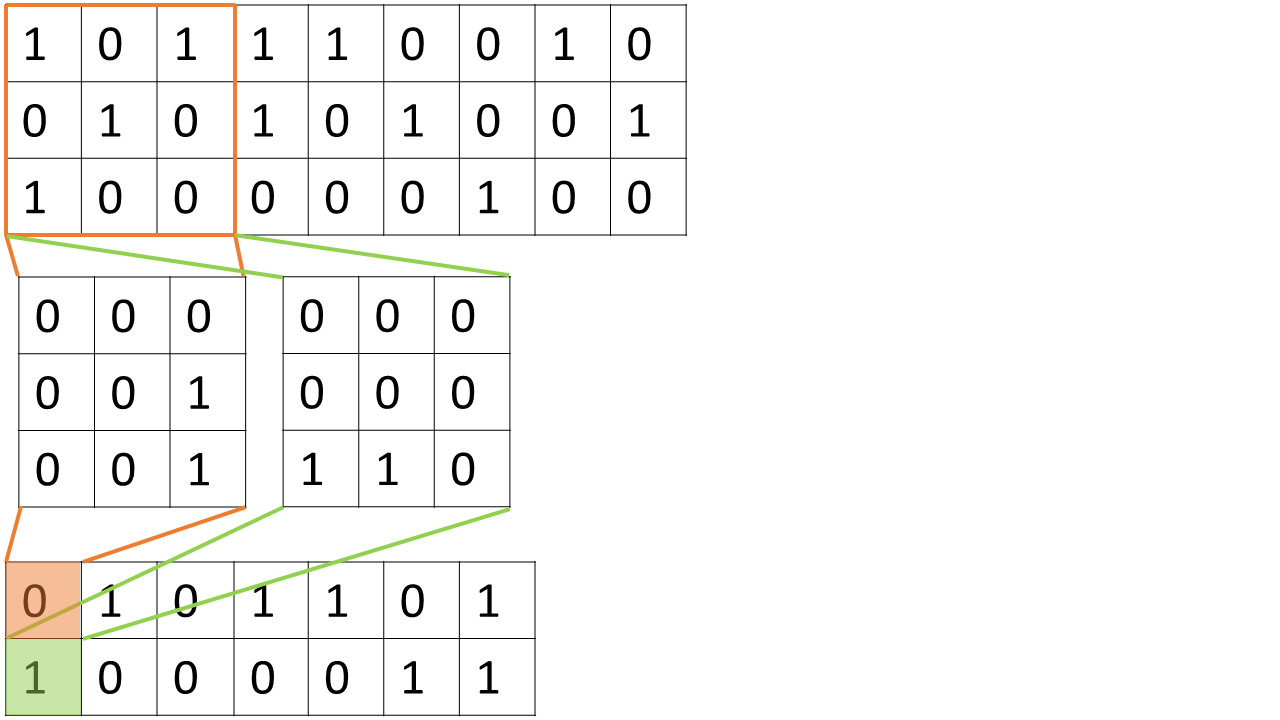
\includegraphics[width=\textwidth]{pictures/Conv2d.png}
%     \caption{Darstellung eines Convolutional Layers mit mehreren Channels.}
%     \label{Conv Layer 2}
% \end{figure}

\threesub{Loss} 

Um zu bestimmen, wie gut ein neuronales Netz ist, gibt es die sogenannte Verlustfunktion (engl. \eng{loss function}), die die Datensätze verwendet, um die Abweichung des Netzwerks vom Ideal zu bestimmen. Diese Abweichung wird auch \eng{loss} genannt.

Trainingsdaten bestehen aus einer Liste aus Trainingsdatensätzen. Jeder dieser Datensätze beinhaltet Eingaben für das Netzwerk und die richtigen Ausgaben dafür. Machine Learning, das mit solchen Trainingsdaten arbeitet, wird Supervised Learning genannt.

Die Funktion für den \eng{loss} der Ausgabeschicht und somit des gesamten Netzwerkes (für einen Datensatz) lautet wie folgt:

\form{ \[
	C_0 = (a_L - y)^2
\]}

%C0 = (aL − y)2 

\noindent wobei $C_0$ der \eng{loss} der Ausgabeschicht, $L$ die letzte Schicht (Ausgabeschicht), $a_L$ der Vektor aller Aktivierungen der Schicht $L$, und $y$ ein Vektor der richtigen Ausgaben für die Eingaben, mit denen die Aktivierungen berechnet wurden, ist. 
	
Um den \eng{loss} zu berechnen, muss man also für alle Neuronen der Ausgabeschicht die Differenz der durchs Netzwerk gegebenen und der in den Datensätzen vorgegebenen Aktivierungen bilden. Danach muss man diese Differenzen quadrieren und am Ende alle Ergebnisse aufsummieren. Dies kann man für alle Testdatensätze wiederholen und von allen \eng{losses} den Durchschnitt nehmen, um die allgemeine Performance eines Netzwerkes zu überprüfen. Diese Art der Verlustfunktion wird mittlere quadratische Abweichung (engl. \eng{mean squared error}, kurz MSE) genannt.
	
Zusammenfassend kann man also sagen, dass der \eng{loss} die Abweichung von den aktuellen Ausgaben des Netzwerkes zu den idealen Ausgaben des Netzwerkes darstellt -- ein perfektes neuronales Netz hätte einen \eng{loss} von 0. Aufgrund der Trainingsdatensätze und der Verlustfunktion weiß man nun, wie stark die Ausgabeschicht abweicht und entsprechend verändert werden muss.

\threesub{Backpropagation}

% Mithilfer der sogenanten Backpropagation werden die Gewichte des Netzwerkes mithilfe der Datensätze angepasst, um den \eng{loss} zu senken.

% Die von uns verwendete Form der Backpropagation ist das simple sogenannte Gradientenverfahren.

% Um die Aktivierungen der Ausgabeschicht anzupassen, müssen alle Gewichte und Biases davor angepasst werden. Um nun zu wissen, wie ein Gewicht verändert werden muss, gibt es beim Gradientenverfahren folgende Funktion:

% \form{\[
% 	\Delta W_{ij} = \epsilon * \delta_i * a_j
% \]}

% Hier ist  $\Delta W_{ij}$ der Wert, um den das Gewicht $W$ zwischen den Neuronen $j$ und $i$ verändert werden muss, $\epsilon$ die Lernrate (meist ein kleiner Wert wie 0.001), $\delta_i$ eine Annäherung der Ableitung des \eng{loss} des Neurons $i$ im Verhältnis zum Gewicht $W_{ij}$, und $a_j$ die Aktivierung des Neurons $j$. Dabei ist oft verwirrend, dass die Schicht des Neurons $i$ aus der Sicht des \feng{forward pass} weiter hinten liegt als die Schicht des Neurons $j$.
	
% % bezeichnet das Neuron, das sich in der vorderen Schicht befindet, und $i$ das Neuron, das sich in der hinteren  (Reihenfolge im \feng{forward pass}), obwohl es bei $W_{ij}$ andersherum steht.

% Für den Bias wird die gleiche Formel benutzt, mit der Ausnahme, dass $a_j$ immer 1 ist und so wegfällt. Der Grund dafür liegt darin, dass der Bias, wie im Abschnitt \hyperref[forward-prop]{\feng{forward pass}} beschrieben, eigentlich nur ein Gewicht ist, das mit einem Neuron verbunden ist, welches immer eine Aktivierung von eins hat.

% Um nun $\delta_i$ für die Ausgabeschicht zu berechnen, gibt es folgende Gleichung: 

% \form{\[
% 	%\delta_i = \sig '\left({\netin}_i\right) * (a_i (\textrm{soll}) - a_i (\textrm{ist})) 
% 	\delta_i = \sig '\left(x_i\right) * (a_i (\textrm{soll}) - a_i (\textrm{ist})) 
% \]}
% wobei $\sig '(x)$ die Ableitung von $\sig(x)$ ist, also $\sig'(x) = \sig(x) * (1 - \sig(x))$, $x_i$ der Netzeingabe des Neurons $i$, $a_i(\textrm{soll})$ die Aktivierung, die das Neuron haben sollte (also das gleiche wie $y$), und $a_i(\textrm{ist})$ die Aktivierung, die das Neuron hat.

% Mit dieser Formel wird berechnet, welche Aktivierung das Neuron haben sollte, was an $a_i(\textrm{soll}) - a_i(\textrm{ist})$ erkennbar ist. Die Aktivierungsfunktion mit der Netzeingabe wird als Faktor mit einberechnet, da möglichst nur die Gewichte stark verändert werden sollen, die bei dem Trainingsdatensatz eine hohe Aktivierung haben, also durch diese Eingaben besonders angesprochen werden. So werden zum Beispiel beim Sortieren nur die Neuronen stark miteinander verknüpft, die für ein bestimmtes Muster verantwortlich sind.

% Für die Neuronen der verdeckten Schichten muss man alle $\delta$'s der nächsten Schicht mit den von dem Neuron dorthin führenden Gewichten multiplizieren und dann summieren. Dadurch werden die Änderungen, die die Aktivierungen dieser Neuronen brauchen ($\delta$), zusammengerechnet, da natürlich die Aktivierungen in der nächsten Schicht unterschiedliche Änderungen in dem gleichen Neuron benötigen.
	
% Durch die Multiplikation mit den dahin führenden Gewichten werden diese Änderungen gewichtet, da sie auf einige Neuronen größere Auswirkungen haben als auf andere. Wie bei der Ausgabeschicht auch wird diese Summe noch mit $\sig'(x)$ multipliziert, um die Aktivierung durch bestimmte Muster angesprochener Neuronen noch weiter zu erhöhen und weniger/kaum angesprochener Neuronen zu senken, sodass die Ergebnisse besser und eindeutiger werden. Die Formel hierfür lautet:

% \form{\[\delta_i = \sig'(x_i) * \sum_{L}{\left(\delta_L\ast W_{Li}\right)}\]}
% \noindent wobei $L$ die nächste Schicht, $\delta_L$ der Vektor aller $\delta$'s der Schicht $L$, und $W_{Li}$ der Vektor aller Gewichte, die ein Neuron der nächsten Schicht und Neuron $i$ verbinden, ist.
% Da immer die (in Reihenfolge des \feng{forward pass} gesehene) nächste Schicht benötigt wird, ergibt es Sinn, diese Optimierung bei der Ausgabeschicht zu starten und dann rückwärts die \mbox{$\delta$-Werte} für jede Schicht zu berechnen und für die nächsten Berechnungen zu speichern -- daher auch der Name Backpropagation.

\subsubsection{Overfitting}

Unterschiede zwischen Testdaten- und Trainingsdaten-Genauigkeit sind ein bekanntes Problem bei neuronalen Netzwerken und werden durch sogenanntes \enquote{Overfitting} verursacht.
Dabei passt sich das Netzwerk zu stark an die Trainingsdaten an, wodurch keine Muster in den Daten gefunden werden können und das neuronale Netzwerk nicht in der Lage ist, neue Daten korrekt zu klassifizieren, da es die Trainingsdaten einfach nur \enquote{auswendig gelernt} hat.  % TODO: Quelle?
 
Oft lässt sich das Problem darauf zurückführen, dass das Erlernen der Generalisierung der Datenerkennung eines neuronalen Netzwerkes darauf basiert, dass es die Trainingsdaten nicht einfach nur Abspeichern und wieder Aufrufen kann, da dies zwar die Kosten minimieren würde, es aber dafür nicht genug \enquote{Speicherplatz} (Komplexität) hat. Also kann Overfitting durch eine zu große Netzwerkstruktur oder zu wenige Daten verursacht werden.
 
Außerdem kann ein schlechtes Signal-Rausch-Verhältnis die Ursache sein: Das Signal-Rausch-Verhältnis gibt an, wie stark sich ein Nutzsignal von dem Hintergrundrauschen abhebt. 
Gerade bei der Datenermittlung mit einem EEG ist dieses Verhältnis sehr schlecht, da die für uns relevanten Signale aus dem Gehirn durch den Schädel und Haut stark abgeschwächt werden, bevor sie bei den Elektroden ankommen. 
Durch großes Hintergrundrauschen ist es für ein neuronales Netz schwer oder sogar unmöglich, grundlegende Muster in den Daten zu finden, da diese womöglich nicht einmal mehr existieren, sodass es durch fehlende Komplexität zwar keine 100\& Genauigkeit durch das direktere Abspeichern der Trainingsdaten erreichen kann, aber die Generalisierung noch schlechter wäre. 
Dadurch tendiert das Modell bei der Kostenoptimierung der Neuronen zum Overfitting.

Um Overfitting entgegenzuwirken, gibt es verschiedene Möglichkeiten. Diese gehören zu den Verfahren der Regularisierung, die ein Modell 
Bei der Verwendung von Dropout (dt. \textit{fallen lassen}) wird einer Schicht des neuronalen Netzwerkes eine Dropout-Wahrscheinlichkeit zugeordnet.
Bei jedem Trainingsschritt des Modells wird dann für jedes einzelne Neuron dieser Schicht basierend auf der Dropout-Wahrscheinlichkeit zufällig entschieden, ob es seinen Wert beibehalten oder auf 0 gesetzt wird. 
Bei einer Dropout-Wahrscheinlichkeit von 30\% werden also im Schnitt 30\% der Neuronen auf 0 gesetzt und somit ignoriert werden.  % Quelle?
Dies führt dazu, dass das neuronale Netzwerk die Daten nicht so einfach auswendig lernen kann. % TODO: weiter ausführen?

Außerdem gibt es die L1- und L2-Regularisierungen.  
Die Idee hinter ist ähnlich zum Dropout, dass sie verhindert, dass das Netzwerk zu komplex wird und sich zu sehr an die Trainingsdaten anpasst.
Im Gegensatz zu \feng{Dropout} wird bei der L2-Regularisierung eine Penalties-Funktion zum Verlust hinzugefügt, die das Ausmaß der Gewichte des Modells beschränkt. Stattdessen wird es gezwungen, eine gewisse Einfachheit beizubehalten, was dazu beitragen kann, dass das Netzwerk besser auf neue, noch nicht gesehene Daten generalisiert.

Die Verwendung von Rauschen (\eng{noise}) auf dem Input für ein Neuronales Netzwerk kann dazu beitragen, das Overfitting zu vermeiden und die allgemeine Robustheit des Modells zu erhöhen.
Die Idee hinter der Verwendung von Rauschen auf dem Input ist, dass das Netzwerk gezwungen wird, sich an zusätzliche Unschärfen in den Eingaben zu gewöhnen und somit besser auf neue, noch nicht gesehene Daten generalisieren kann. Durch die Erhöhung der Robustheit des Modells gegenüber kleinen Änderungen der Eingaben kann es auch weniger empfindlich auf kleine Störungen oder Verzerrungen in den Daten reagieren.

\section{Ergebnisse}

Der gesamte Quellcode unseres Projektes sowie alle gesammelten Daten lassen sich auf unserem GitHub Repository \cite{InterpretingEEG} finden.

Wir werden in diesem Bericht nur einige Design-Konzepte unseres Programms erklären; Informationen über die Verwendung sowie Details lassen sich in unserer Software-Dokumentation \cite{BCIInterfaceDocs} finden. 

\subsection{Nutzerfreundlichkeit}

Im Gegensatz zu letztem Jahr, in dem unser Programm eher die Funktion eines Proof-of-Concept erfüllte, haben wir dieses Jahr den Fokus viel stärker auf Nutzbarkeit und Anpassbarkeit unseres Programms gelegt.

\subsubsection{Verwaltung}

Letztes Jahr war es für die Verwendung unseres Programms notwendig, die einzelnen Dateien herunterzuladen und direkt zu inkludieren.
Es gabe keine Versionskontrolle, keine einfache Methoden zum Aktualisieren und die Verwaltung der Abhängigkeiten des Programms hat ebenfalls nicht automatisch funktioniert.

Aber dieses Jahr haben wir das Framework als tatsächliches Julia-Paket entwickelt, welches über die normale Paketverwaltung verwaltet werden kann, und haben dadurch diese Probleme gelöst (s. \coderef{code:Verwaltung}).
Alle von dem Paket benötigten Abhängigkeiten werden automatisch installiert und mitverwaltet.

% TODO: test
\begin{code}[0.75]{Verwaltung unseres Pakets in einem Skript; die Verwendung der Julia REPL ist ebenfalls möglich.}{code:Verwaltung}
    using Pkg
    # Paket installieren
    Pkg.add("https://github.com/AR102/Interpreting-EEG-with-AI")
    # Paket aktualisieren
    Pkg.update("BCIInterface")
    # Paket in einem Programm verwenden
    using BCIInterface
\end{code}

\subsubsection{Erweiter-- und Anpassbarkeit}

Wir haben beim Design des Frameworks starken Gebrauch von der Multimethoden-Unterstützung von Julia gemacht.
Dabei können mehrere Funktionen den gleichen Namen haben. Welche Funktion ausgeführt wird, ist abhängig von der Anzahl und den Typen der Argumente. Für ein Beispiel siehe \coderef{multipleDispatch}.

\begin{code}{Multiple-Dispatch-Beispiel}{multipleDispatch}
# eigenen Datentypen namens "Dog" definieren
struct Dog end
# eigenen Datentypen namen "Cat" definieren
struct Cat end

# Funktion wird ausgeführt, wenn Parameter vom Typ "Dog" ist
makenoise(animal::Dog) = println("Wuff!")
# Funktion wird ausgeführt, wenn Parameter vom Typ "Cat" ist
makenoise(animal::Cat) = println("Meoow!")
\end{code}

Da wir unser Programm modular aufgebaut haben, ist es durch Multimethoden leicht möglich, einzelne Aspekte anzupassen, indem man eigene Typen definiert und dann die intern verwendeten Funktionen, an die diese Typen weitergereicht werden, \enquote{überlädt} (neue Multimethoden definiert). Dies ermöglicht eine leichte Erweiterung und Anpassbarkeit unseres Frameworks.

Ein Beispiel davon ist in \coderef{code:customEEG} zu sehen, wo ein eigenes EEG Gerät verwendet wird. In diesem Beispiel gibt dieses \enquote{EEG} nur zufällige Werte aus, aber der Nutzer könnte in der Funktion \mintinline{julia}{get_voltage} etwas beliebiges schreiben, also auch sich mit dem Internet verbinden, USB-Ports ansteuern, auf einen Netzwerk-Stream zugreifen, etc. 

Ein großer Vorteil dieser Vorgehensweise ist, dass man als Nutzer weder auf Funktionen des Pakets verzichten / diese selbst implementieren muss noch den Quellcode unseres Pakets anpassen muss, was aufwändig sein und zu Problemen mit Paketaktualisierungen sowie Übersicht führen könnte. 

\begin{code}{Beispiel für die Verwendung eines eigenen EEGs}{code:customEEG}
using BCIInterface
# eigenes EEG Gerät als eigenen Datentypen definieren
struct MyBoard <: BCIInterface.EEG.EEGBoard
    # data_descriptor beschreibt Form der Daten
    # (Anzahl Elektroden? rohe Daten? Frequenzen?)
    data_descriptor::DataDescriptor
end
NUM_CHANNELS = 8
MyBoard() = MyBoard(RawDataDescriptor(NUM_CHANNELS))
# Überlade die interne Funktion zum Abrufen von Daten
function BCIInterface.EEG.get_voltage(board::MyBoard, channel::Int)
    # gib zufällige Zahl zwischen 0 und 1 zurück
    return rand()
end

device = Device(MyBoard(NUM_CHANNELS)
...
\end{code}

\subsubsection{Weiteres}

Weiter haben wir bei der Verwaltung der EEG-Daten ein einfaches Interface zum Speichern, Abrufen und Filtern von Daten implementiert.
So können mit den Daten auch noch \enquote{tags} und \enquote{extra info} gespeichert werden, die später für die Filterung und Verarbeitung der Daten sehr nützlich sein können, wie es \coderef{code:tags} zeigt.

% TODO: update if not implemented in time

\begin{code}{Geürztes Beispiel, das die Verwendung von \enquote{tags} und \enquote{extra info} zeigt}{code:tags}
...
save_data(experiment, tags = [:room102, :PersonA], 
    extra_info = Dict(:temp => 22.3))
...
filter = DataFilter(
    tags = [:PersonA], # nur Daten von Person A
    nottags = [:room105], # keine Daten aus Raum 105
    extra_filter = x -> x.temp < 21 # nur Daten, wo Temperatur unter 21 war
)
filter!(data, filter)
...
\end{code}
\subsection{Framework}

Unser Ziel war es, ein Framework zu entwickeln, das einfach zu benutzen ist und einem Zeit bei der Entwicklung von BCIs erspart. Dafür haben wir ein eigenes Julia-Package geschrieben, mit dem man einfach Daten aufnehmen und speichern sowie ein eigenes neuronales Netzwerk erstellen und in einer Live-Anwendung testen kann.

Dieses Package haben wir anschließend getestet, indem wir es genutzt haben, um ein BCI zu entwickeln, welches erkennen kann, ob man gerade an die Richtung rechts oder an die Richtung links denkt. Diese Klassifizierung ist relativ komplex, da dabei kein einfacher Ausschlag oder Anstieg einer bestimmten Frequenz verursacht wird, anders als z.B. beim Blinzeln oder einem akustischem Signal. Deswegen ist es für einen Menschen auch fast unmöglich, nur anhand der Daten des EEGs manuell festzustellen, ob eine Person gerade an eine bestimmte Richtung denkt.

Um herauszufinden, ob es überhaupt möglich ist mit unserem EEG, das nur 4 Elektroden besitzt, Gedanken an verschiedene Richtungen zu klassifizieren, haben wir zuerst ein neuronales Netz mit Daten, die wir im Internet gefunden haben, trainiert. Diese Daten wurden mit einem 16 Elektroden EEG aufgenommen. Nachdem wir unser Modell mit diesen Daten trainiert haben, haben wir eigene Daten aufgenommen, um zu testen, ob sich dieses Modell auch auf Daten generalisieren lässt, die mit unserem EEG aufgenommen wurden.

Wir waren in der Lage, eine sehr gute Genauigkeit beim Testen des Modells mit Trainingsdaten zu erreichen. 
% TODO: Graph? Zahlen?
Mit der Genauigkeit ist gemeint, welchen Anteil der gegebenen Datensätze das neuronale Netzwerk korrekt klassifizieren konnte. 
Da die Trainingsdaten dem Modell durch das Trainieren jedoch bereits bekannt waren, haben wir zusätzlich noch die Genauigkeit des Modells bei der Analyse der Testdaten bestimmt. 
Diese wurden vorher nie zum Trainieren des Netzwerks verwendet und repräsentieren somit viel besser die Genauigkeit des Modell in der späteren Verwendung, wo das Modell mit unbekannten, neuen Umständen und neuen, noch nie zuvor gesehenen Daten klarkommen muss. % TODO: Quelle?

Die Genauigkeit lag jedoch bei den Testdaten bei ungefähr ... %TODO
und somit deutlich niedriger als bei den Trainingsdaten. 
Dieses starke Overfitting lässt sich wahrscheinlich auf das schlechte Signal-Rausch-Verhältnis zurückführen, das durch die Datenermittlung mit einem EEG entsteht. Man kann also festhalten, dass unsere neuronales Netz zwar besser als zufällig ist, aber trotzdem noch keine sichere Erkennung liefert.

\section{Diskussion}

Ziel unseres Projektes war es, ein Framework zu entwickeln, welches sich leicht auf die eigenen Zwecke anpassen lässt und das entwickeln von BCIs vereinfacht. Dies haben wir mit unserm eigenen Package erreicht, da es Entwicklung in einer stark abstrahierten Form ermöglicht und aufgrund unserer ausführlichen Dokumentation auch für Anfänger geeignet ist.

TODO:
\begin{itemize}
    \item Hyper Parameter Optimization
    \item Mehr Standard Parameter-Sätze
    \item Integration \& Testen des Selbstbau-EEG
    \item Vergleich Sentdex, unser Ganglion und Selbst-Bau
\end{itemize}

\section{Quellen}
\subsection{Abbildungen}
\begin{table}[h!]
    % Abstand zwischen Tabellenzeilen
    \renewcommand*{\arraystretch}{1.2}
    \centering
    {
    \setlength{\tabcolsep}{0pt}
    \begin{tabular}{p{0.08\linewidth}p{0.9\linewidth}}
        Abb. \ref{fig:conv_layers} %
        & Kopiert und abgeändert von \href{https://tikz.net/conv2d/}{https://tikz.net/conv2d/}, ursprünglicher Author ist Janosh Riebesell  \\
        % Abb. \ref{fig:dense_nn} %
        % & Kopiert und abgeändert von \href{https://tikz.net/regular-vs-bayes-nn/}{https://tikz.net/regular-vs-bayes-nn/}, ursprünglicher Author ist Janosh Riebesell \\
        Abb. \ref{fig:OPV} %
        & Linker Teil: \href{https://www.conrad.de/de/ratgeber/handwerk-industrie-wiki/elektronik-bauteile/lm393.html}{https://www.conrad.de/de/ratgeber/handwerk-industrie-wiki/elektronik-bauteile/lm393.html}, Rechter Teil: \href{https://www.reichelt.de/operationsverstaerker-2-fach-dip-8-lm-358-dip-p10483.html?CCOUNTRY=445\&LANGUAGE=de}{https://www.reichelt.de/operationsverstaerker-2-fach-dip-8-lm-358-dip-p10483.html?CCOUNTRY=445\&LANGUAGE=de}\\
    \end{tabular}
    }
    \label{tab:my_label}
\end{table}
\printbibliography[title={Literatur}, keyword={Literatur}]
\printbibliography[title={Anderes}, notkeyword={Literatur}]
\end{document}